\chapter{User Guide}

\section{Instructions}
% You must provide an adequate user guide for your software. The guide should provide easily understood instructions on how to use your software. A particularly useful approach is to treat the user guide as a walk-through of a typical session, or set of sessions, which collectively display all of the features of your package. Technical details of how the package works are rarely required. Keep the guide concise and simple. The extensive use of diagrams, illustrating the package in action, can often be particularly helpful. The user guide is sometimes included as a chapter in the main body of the report, but is often better included in an appendix to the main report.

The following guide provides instructions on how to use EasyAPI to create an API.

\subsection{Setting up the environment}

In order to run this project on your machine, follow these instructions:

\begin{enumerate}
\item  Ensure you have Python 2.6+/3.3+ installed
\item If you haven't got pip installed, follow the instructions on the \href{https://pip.pypa.io/en/stable/installing/}{official pip installation page}
\item Run the command "pip install --ignore-installed -U spacy" in Terminal/Command Line to install Spacy
\item Run the command  "python -m spacy download en" to download the English corpus in Spacy. This may take over 30 minutes depending on the internet connection
\item If you have any issues following the two above instructions, please refer to the  \href{https://spacy.io/docs/usage/}{official instructions on the Spacy website}
\item Install PostgreSQL by following the steps on the \href{https://www.postgresql.org/download/}{official website}
\item Install Node.js from the download links \href{https://nodejs.org/en}{in the official website} (this will also install NPM)
\item Install Flask with the command "pip install flask"
\item Install the Node.js environment runners with the command "npm install -g neutrino react-scripts"
\item Run the PostgreSQL server and note the connection details
\item In the file "backend/src/config/connections.js", enter your connection details
\item Install the dependencies for the back-end with the command "npm install" while in the ``./backend'' directory
\item Install the dependencies for the front-end with the command "npm install" while in the ``./frontend'' directory
\item Run the python server with the command "python backend/src/nlp/index.py"
\item In a seperate Terminal/Command Line process, run the back-end server with the command "npm start" while in the ``./backend'' directory
\item In a seperate Terminal/Command Line process, run the front-end server with the command "npm start" while in the ``./frontend'' directory
\item Open "http://localhost:3000/" in a web browser and the application will appear
\end{enumerate}

If you have issues running any of the commands above, try prefixing them with the ``sudo'' command. This will run them in an administrative mode.

\subsection{Creating an account}
When you first open the EasyAPI web application, you will be presented with an authentication screen. Here you will be asked to either create a new account or login with an existing one.

Since this is the first time, enter a username and a secret password into the text fields. Afterwards, click on the ``Next'' bellow.

If you receive any errors, simply adjust either your username or password to match the criteria.

\begin{figure}
\label{login}
\centerline{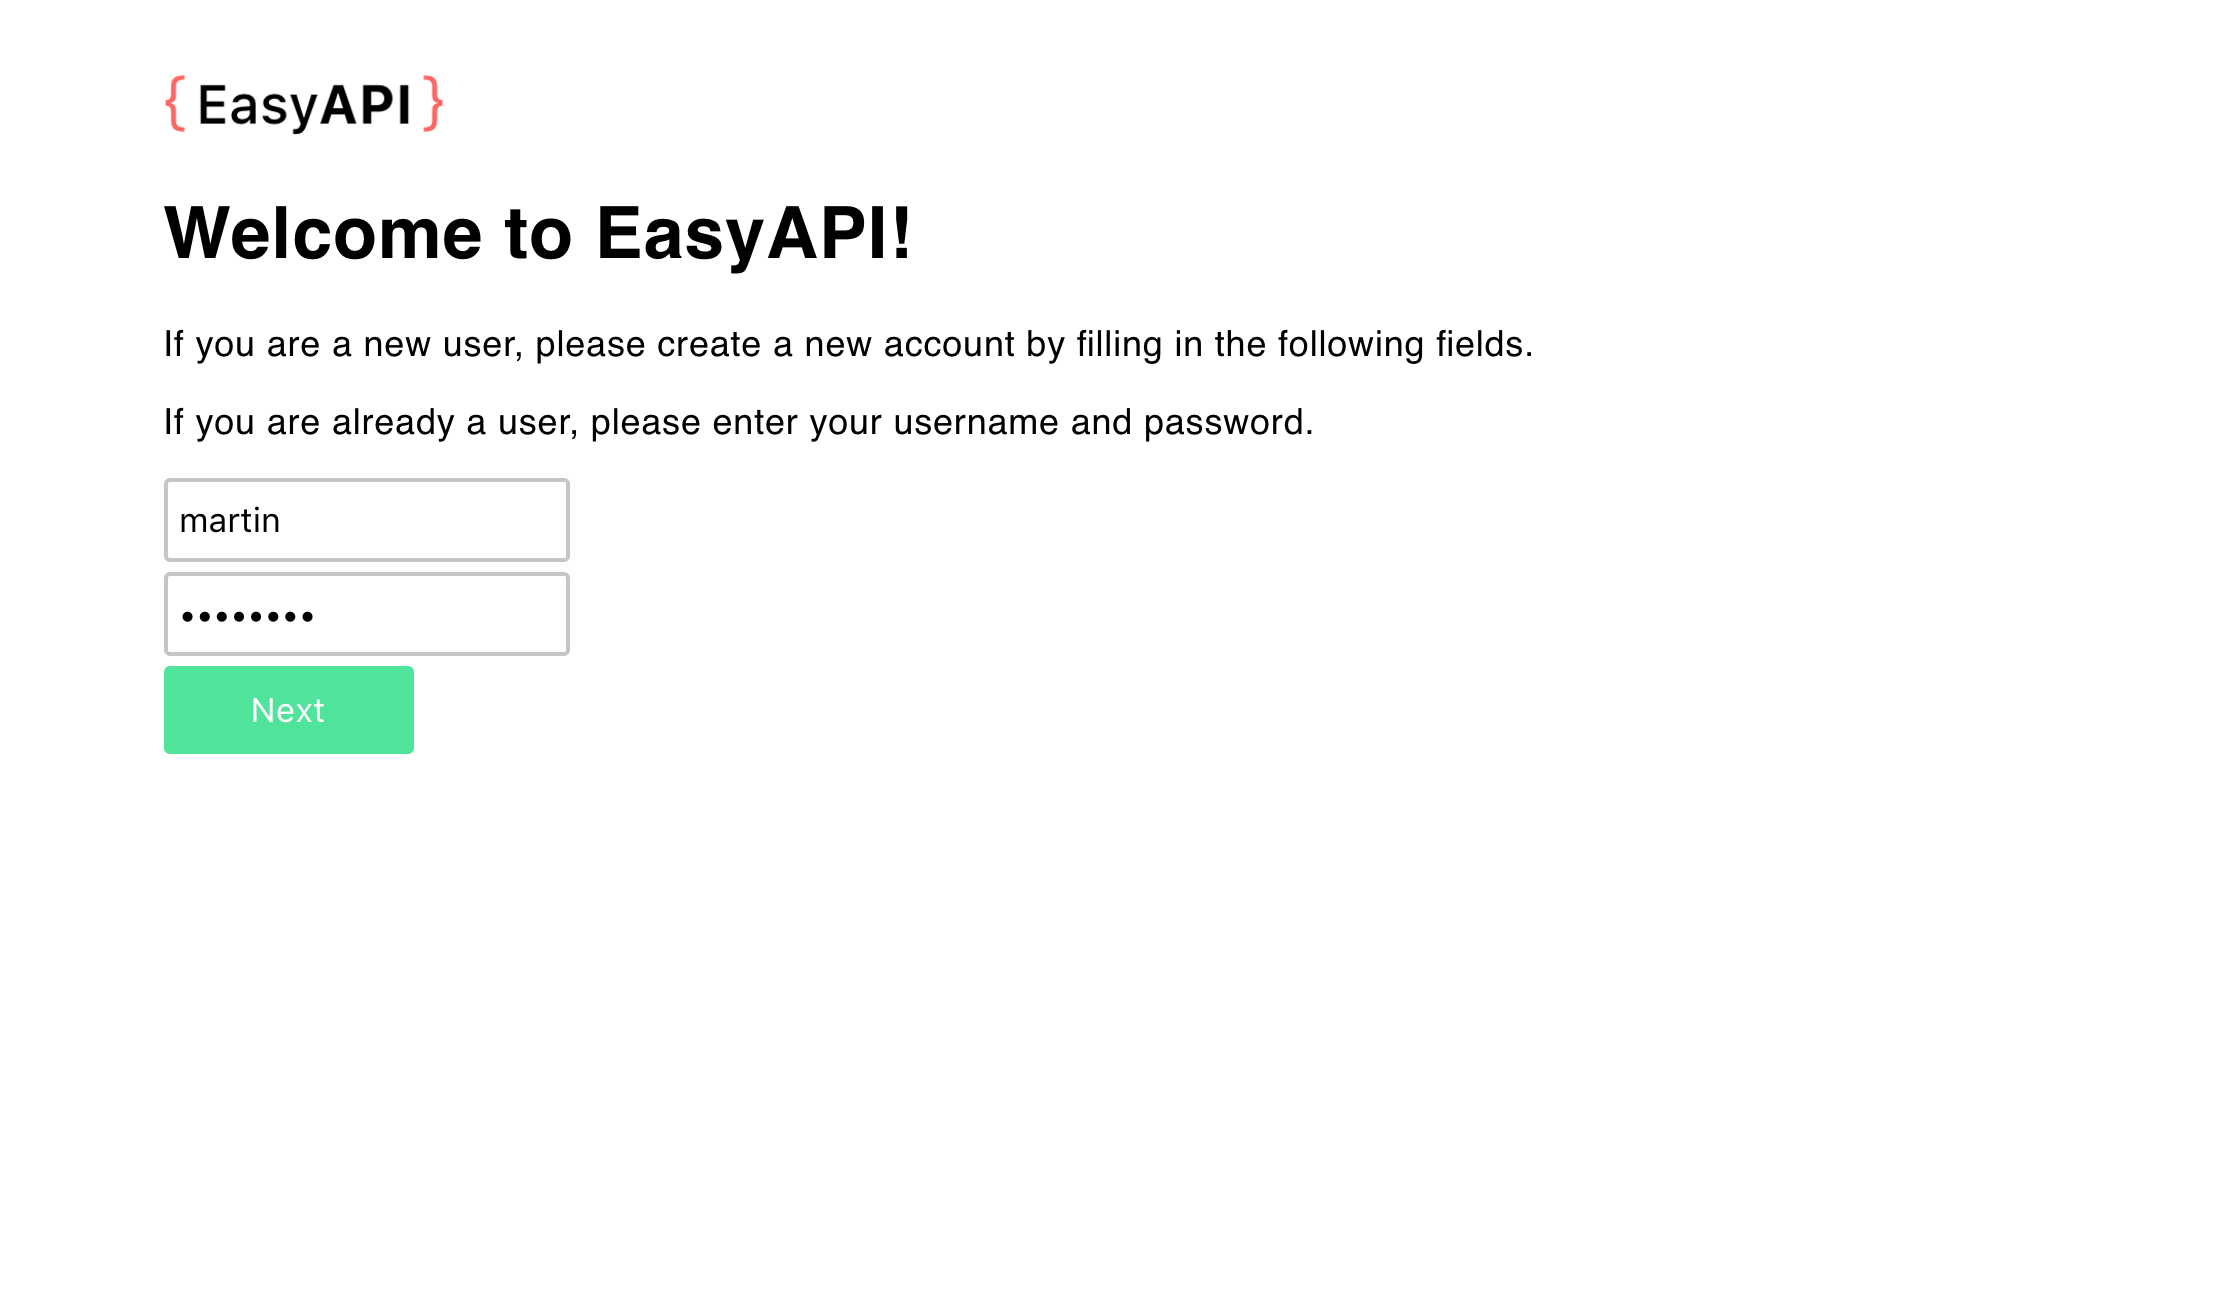
\includegraphics[scale=0.4]{screenshots/login.png}}
\caption{The authentication screen}
\end{figure}

\subsection{Logging in with an account}
If you are returning to the application with an existing account, you can use the authentication screen to login. Simply enter the email and password you used previously into the text-fields. The system will detect that these details were used before and will authenticate you.


\subsection{Creating a new API}
After successful authentication you should be transferred to the API List screen. Here you can view and modify existing APIs and also create new ones.

To create a new API, click on the green plus button. This will transfer you to the setup screen where you can continue creating your API.


\begin{figure}
\label{servicelist}
\centerline{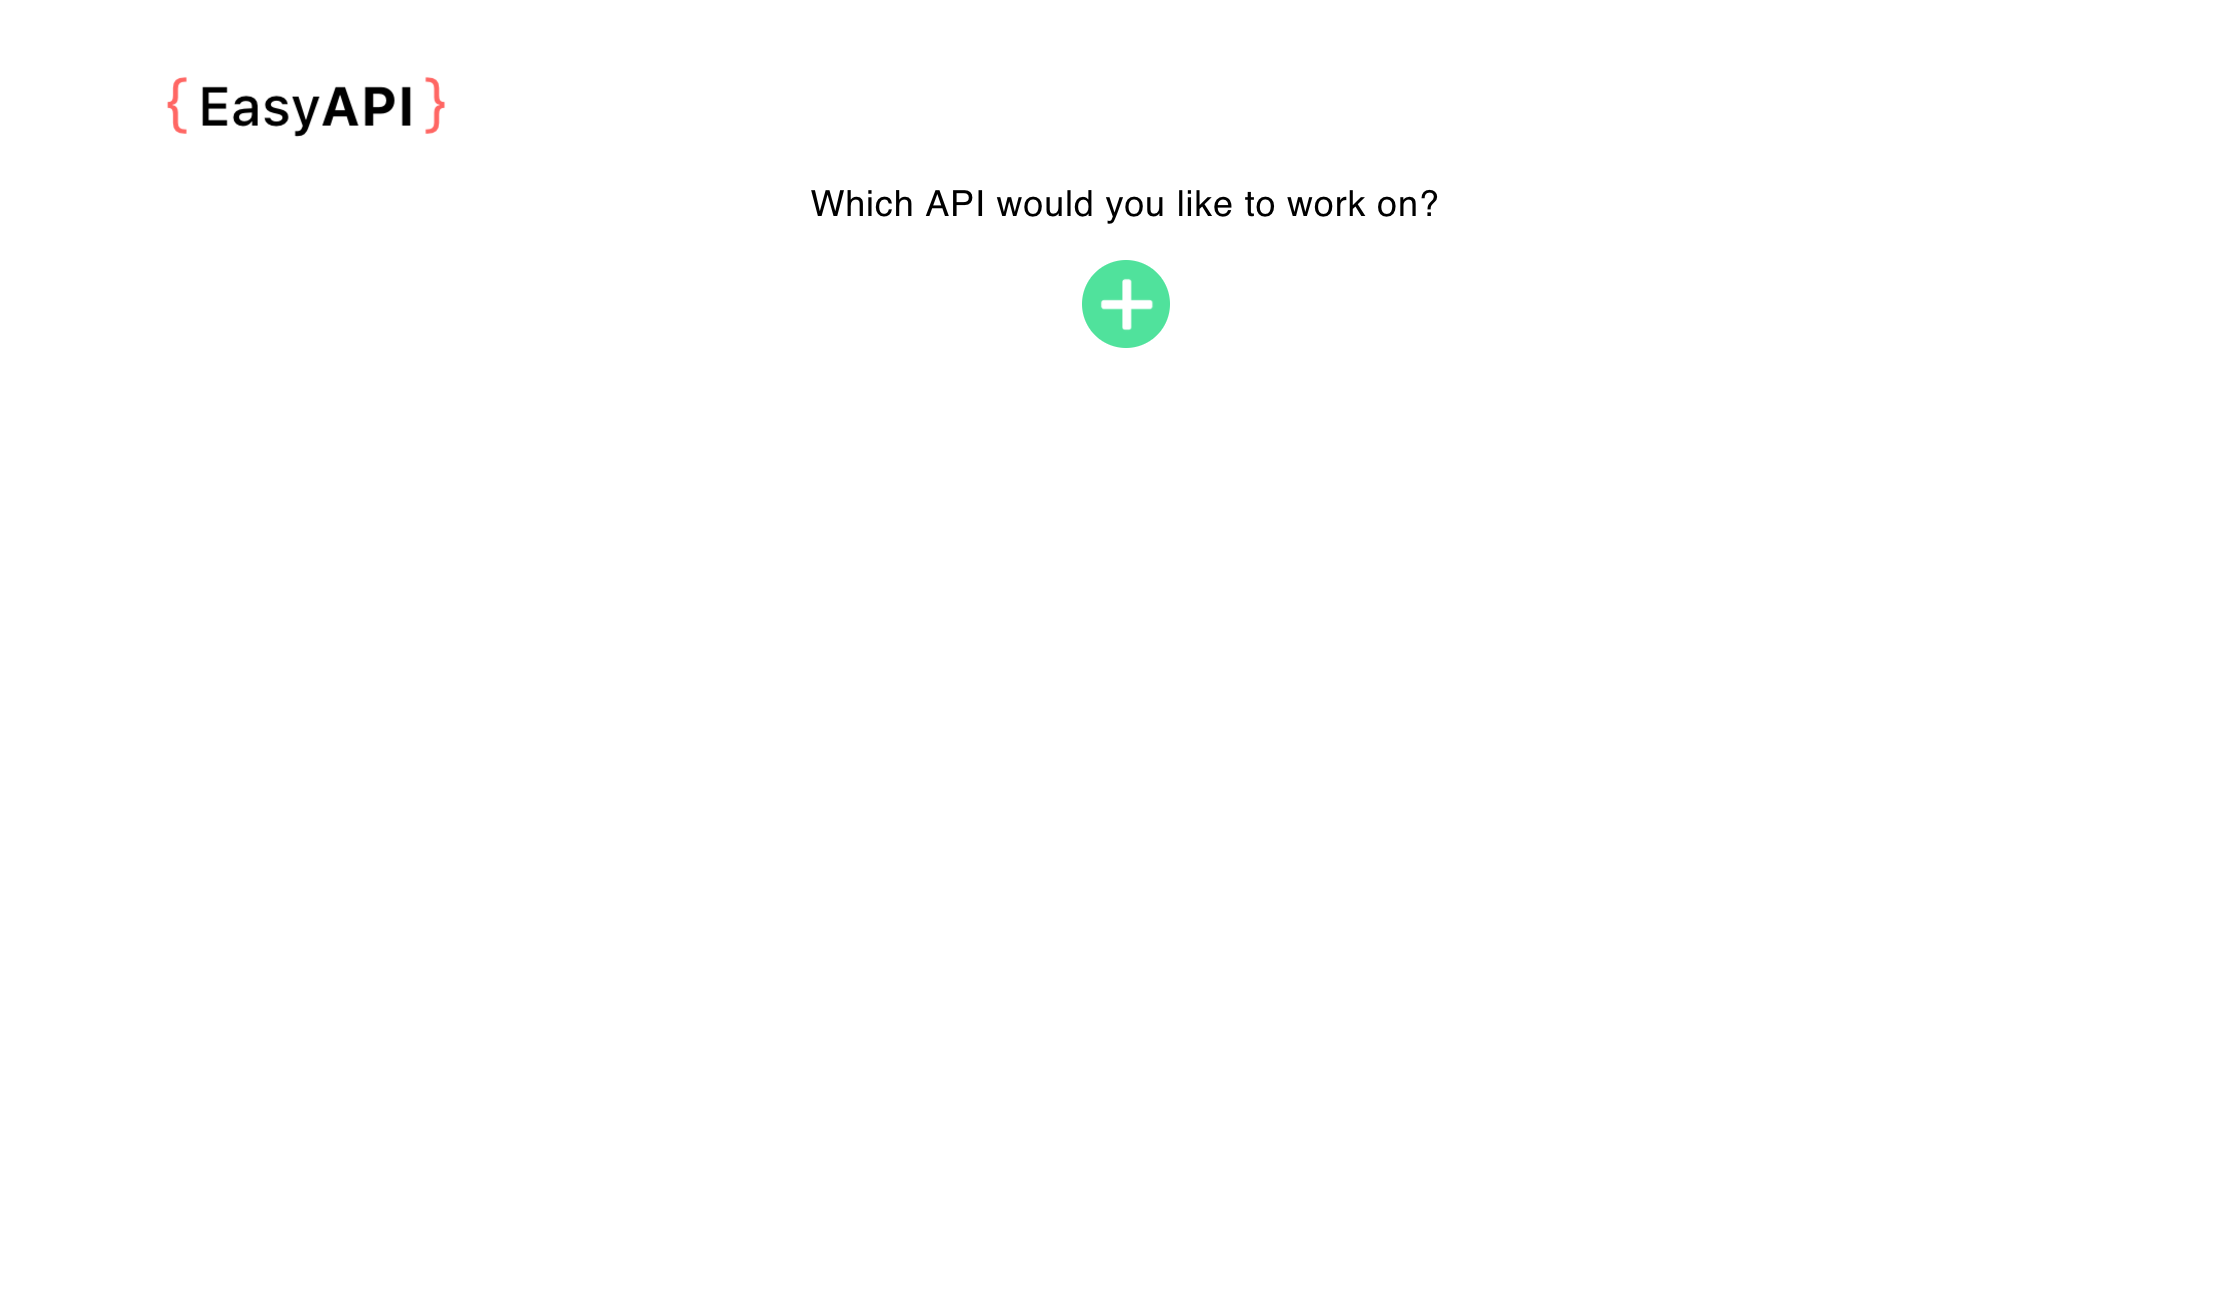
\includegraphics[scale=0.4]{screenshots/servicelist.png}}
\caption{List of APIs screen}
\end{figure}


\subsection{Creating a new API with a domain description}
Once you are on the setup screen, you can follow the instructions to create your API.

We will now build an API from a domain description. In the first screen, you are asked to enter a name for the API. Think of a 1-3 word title which effectively sums up your domain. For example, if we want to create an API for a Pet store, we can use the name ``Pet Store''. After entering the name, click on the ``Next'' button.


\begin{figure}
\label{name}
\centerline{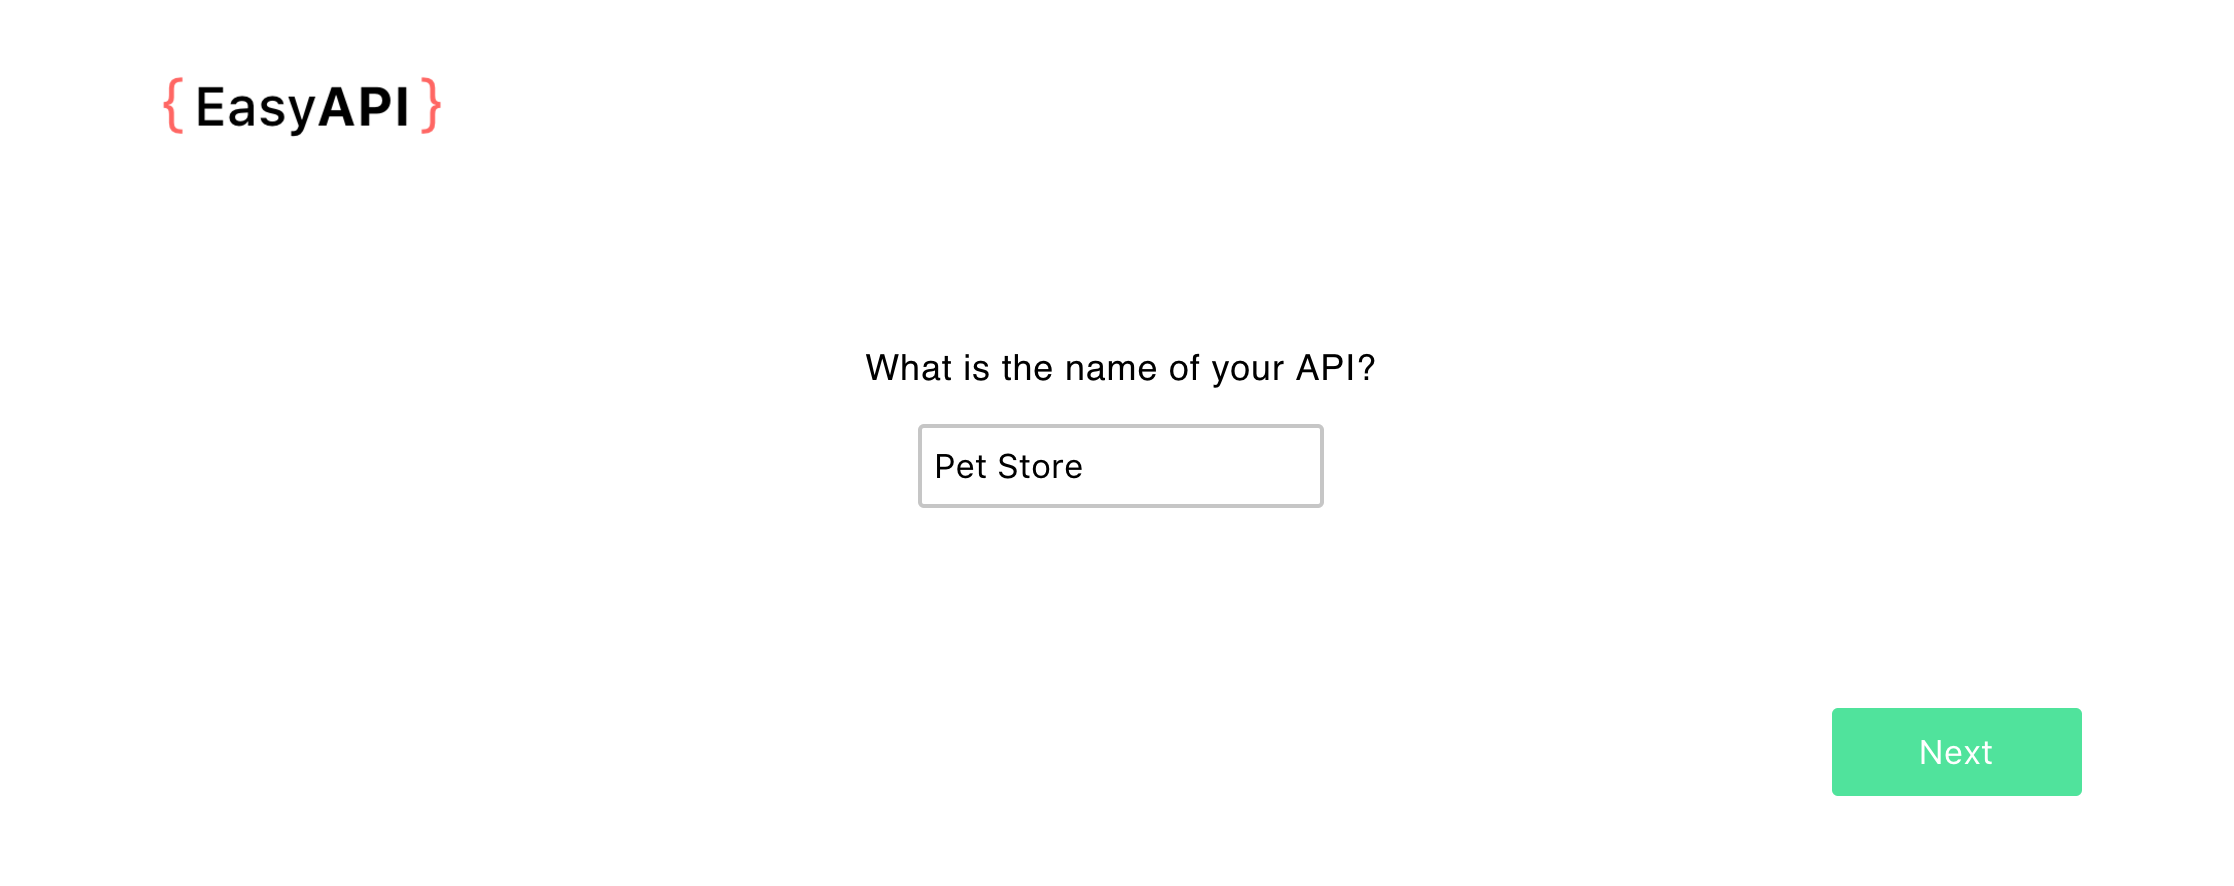
\includegraphics[scale=0.4]{screenshots/name.png}}
\caption{Name selection screen}
\end{figure}



In the second screen, you will be asked to select how you want to create your API. Here we have two options: from a domain description or spreadsheet. In this case we want to create it from a domain description, therefore select the option by clicking on the ``From scratch'' option. Once it is selected, you can click on the next button.

\begin{figure}
\label{methodscratch}
\centerline{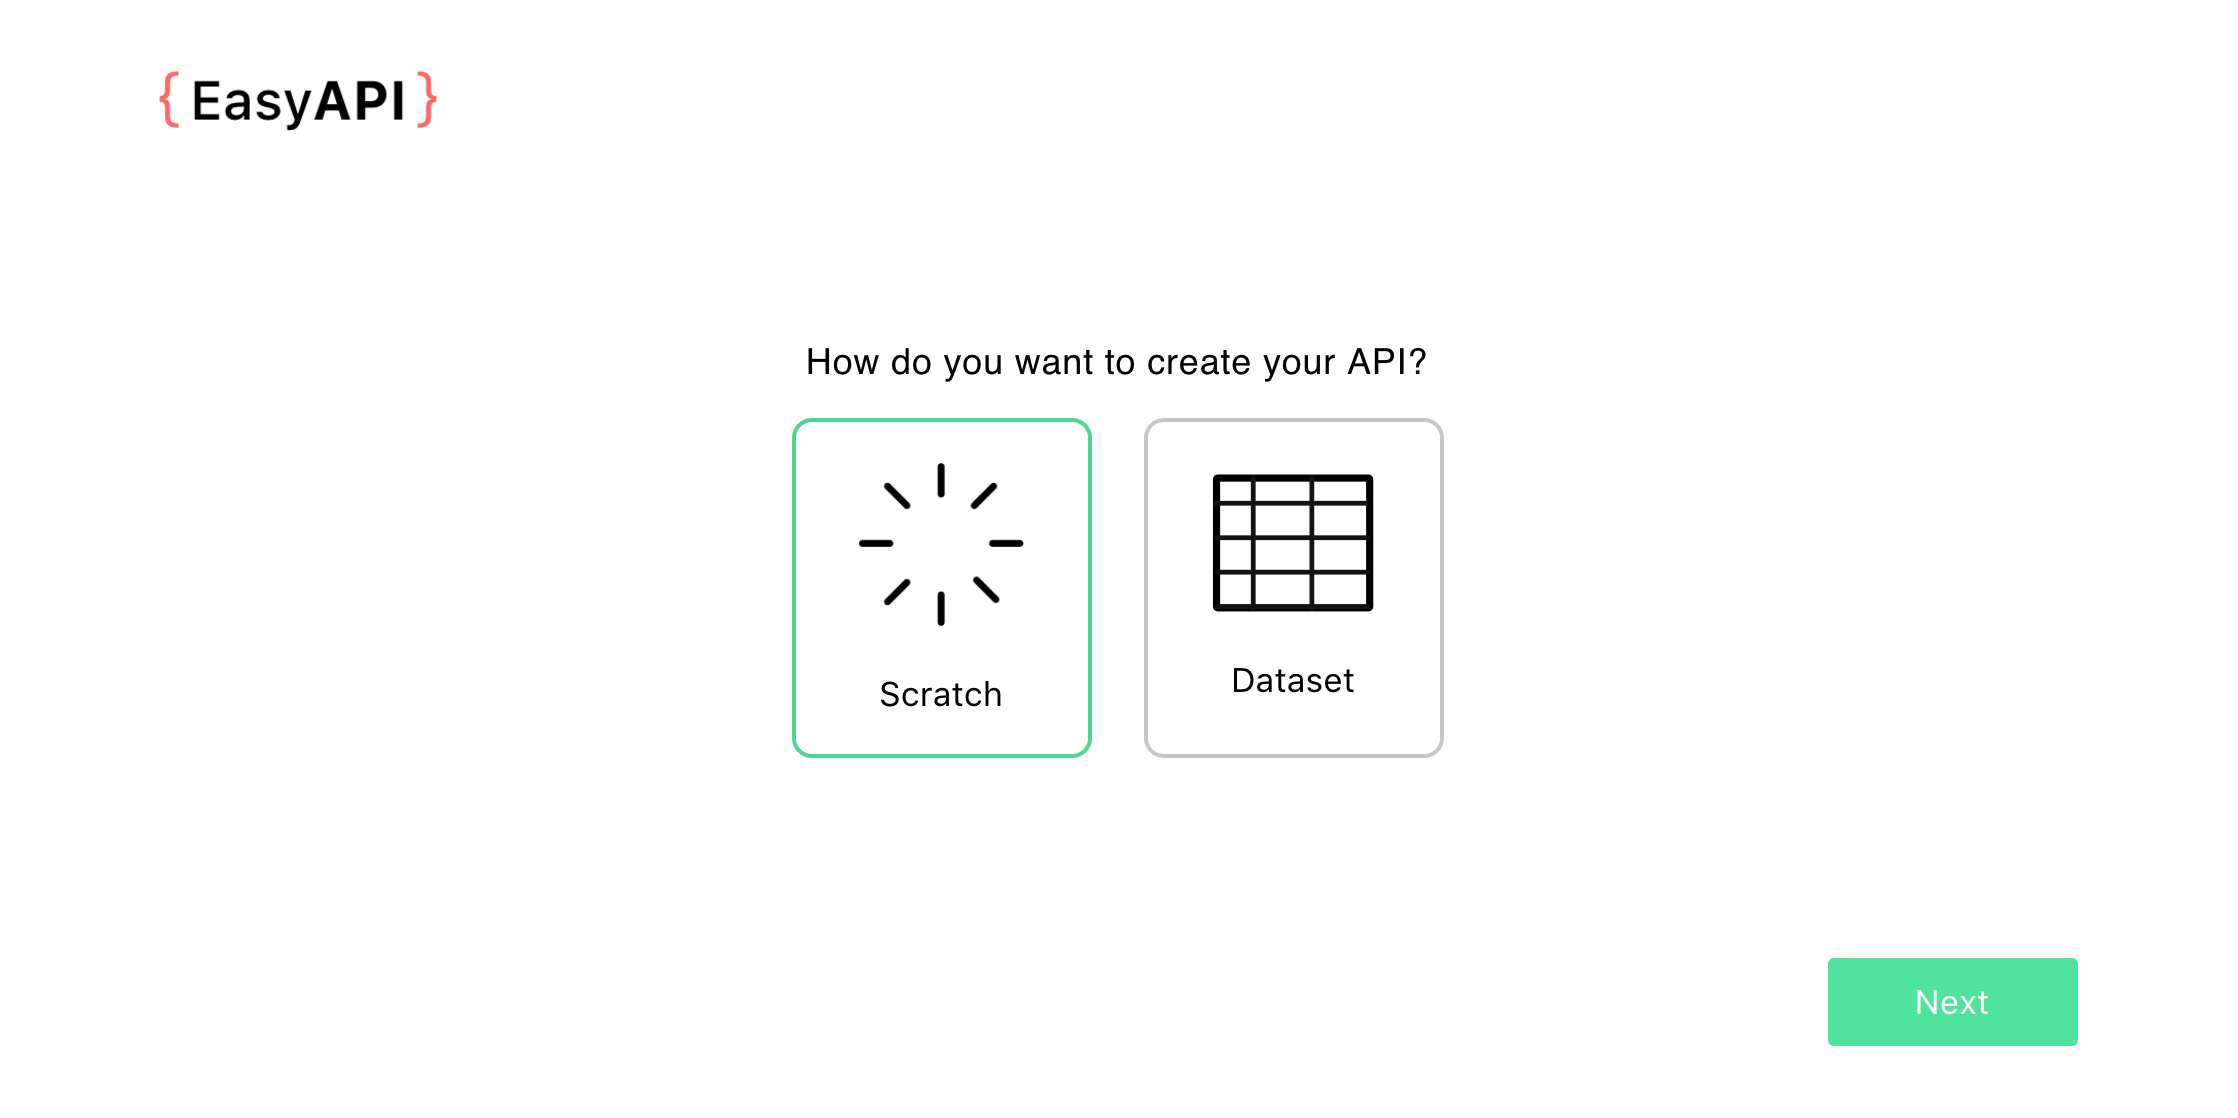
\includegraphics[scale=0.4]{screenshots/methodscratch.png}}
\caption{Method selection screen}
\end{figure}


Finally, we will be presented with a textbox where we can enter our domain description. In order for EasyAPI to extract the correct definition, it is best to describe the domain directly. One-by-one describe all the various entities that are in your domain, with their respective attributes and relationships.



\begin{figure}
\label{naturalimg}
\centerline{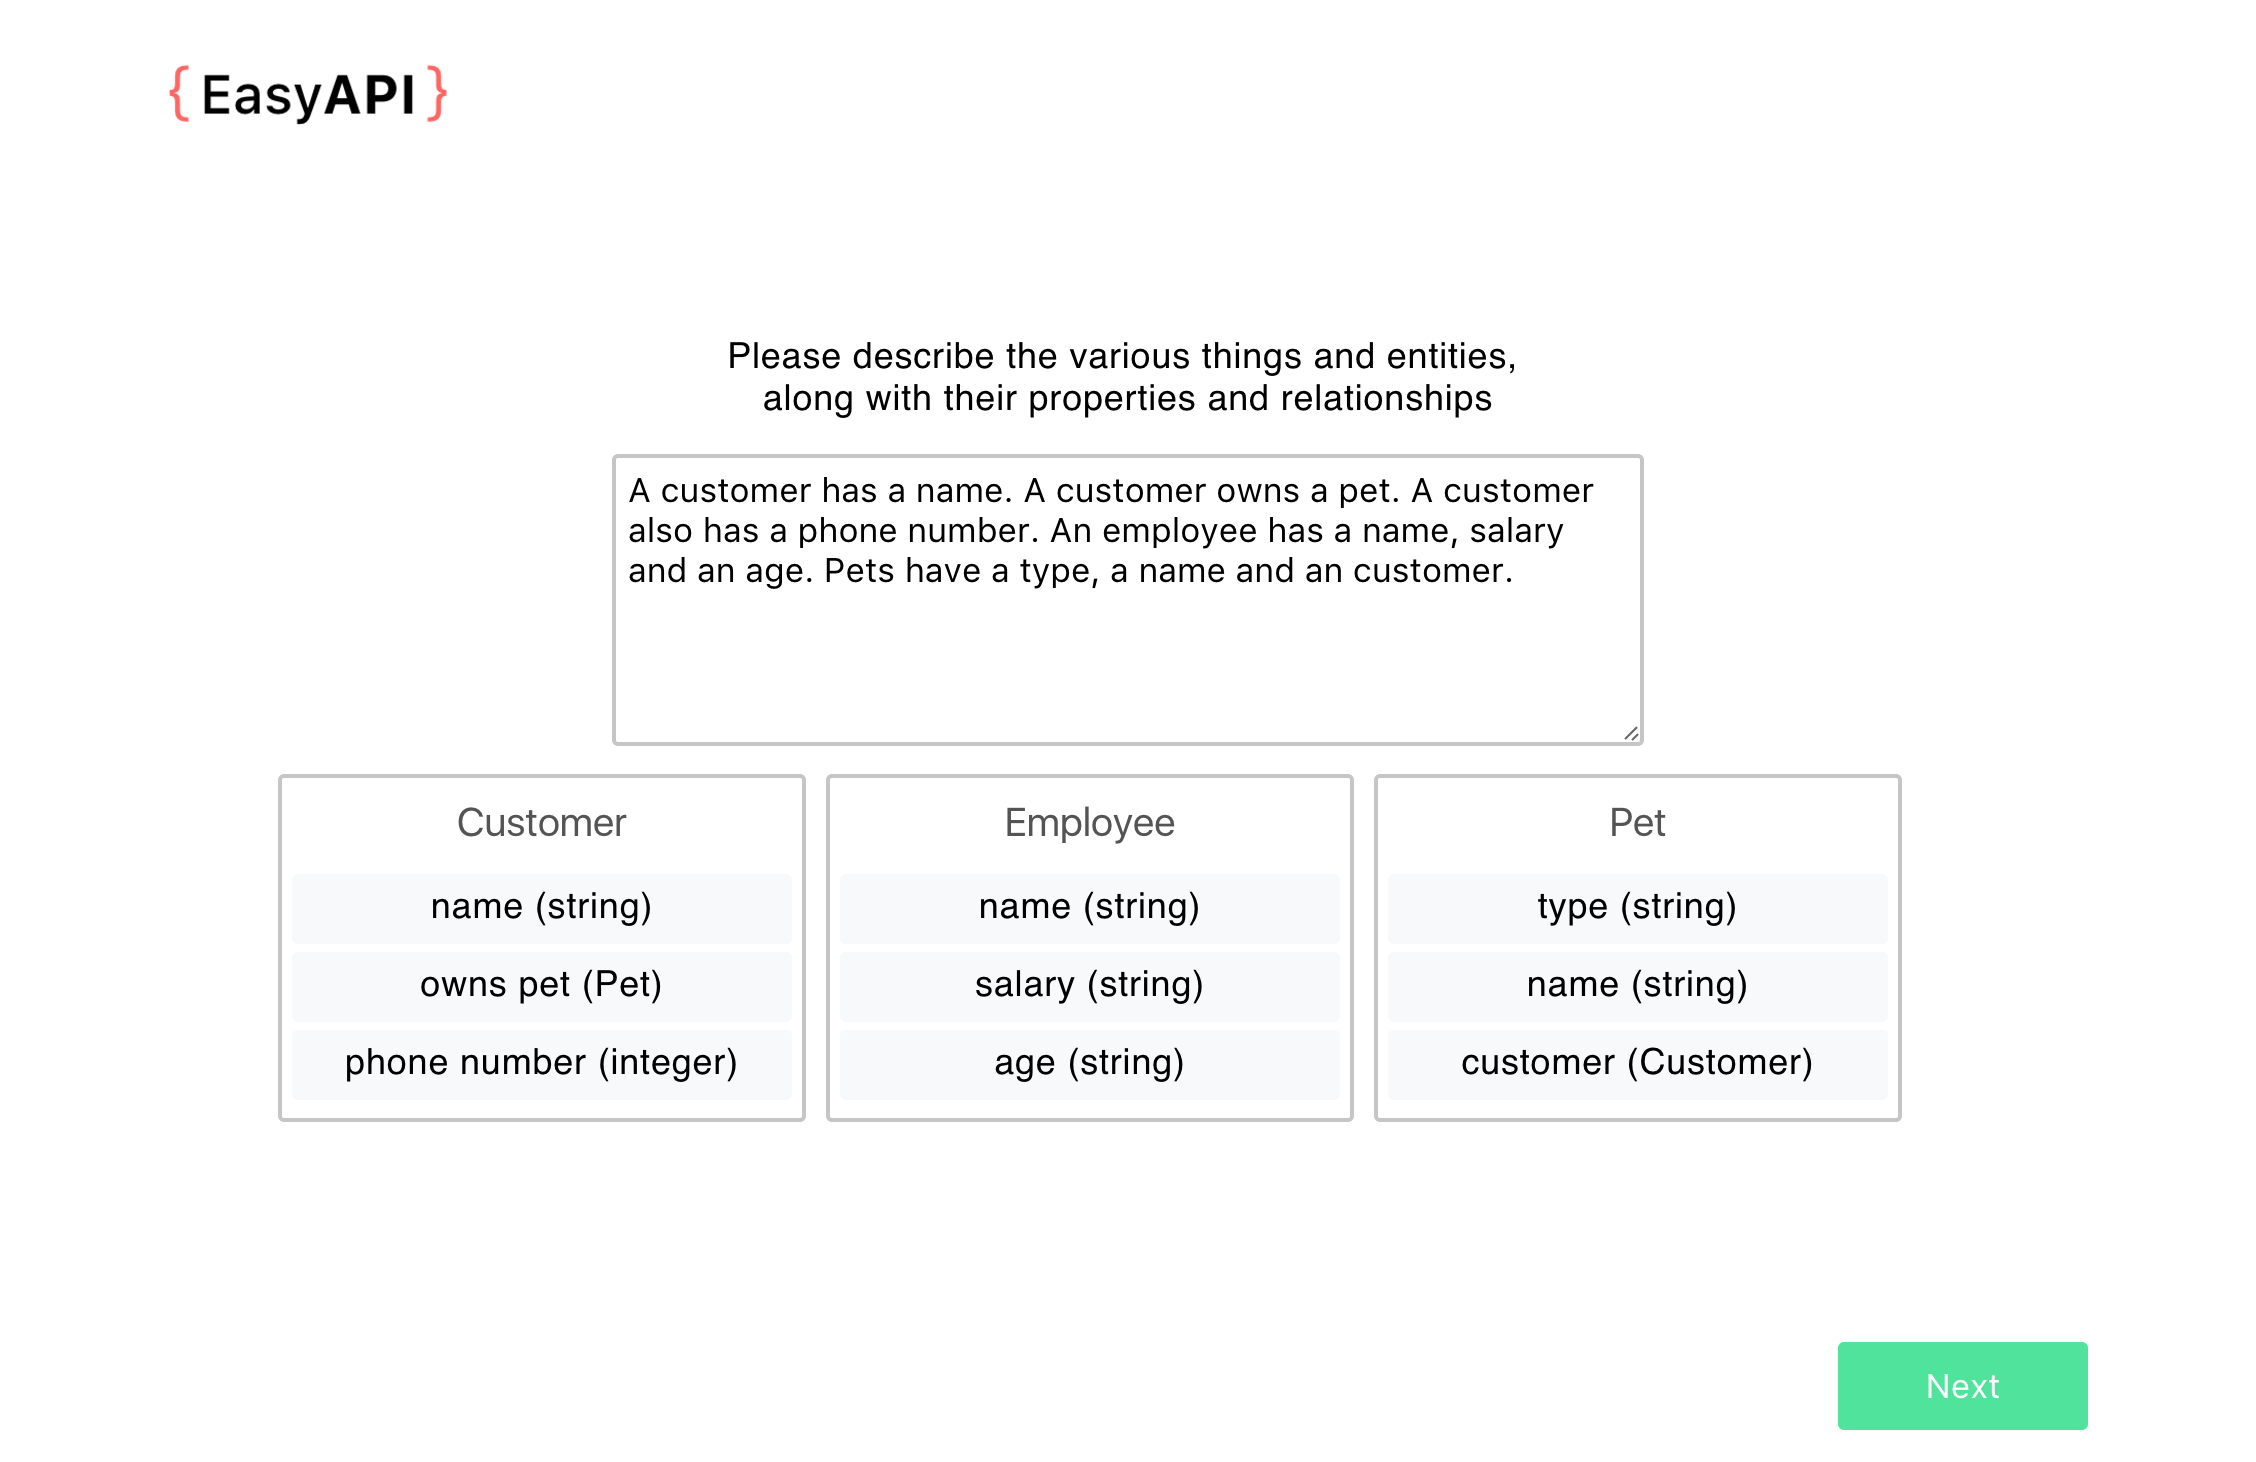
\includegraphics[scale=0.4]{screenshots/natural.png}}
\caption{Setup from scratch screen}
\end{figure}




For our pet store example, we may want to model a Pet store. We want to store information about our customers, employees, and our pets. This would be an appropriate domain description for those entities:

\blockquote{A customer has a name. A customer owns a pet. A customer also has a phone number. An employee has a name, salary and an age. Pets have a type, a name and an customer.}

When you type, the system will preview the model definition that was extracted from your description. If you think that something has been incorrectly parsed, try to rephrase it in simpler, clearer terms. If it still fails to correctly infer your domain description, in the next screen you will be able to modify it manually.

\subsection{Creating a new API with a spreadsheet}
If you already have a spreadsheet containing data which you would like to convert to the API, you can do so directly in the setup.


After creating a new API in the service list screen and typing the name of the API, select the spreadsheet from the creation methods. Afterwards, click on the "Next" button, which will transfer you to the spreadsheet setup screen.


In this screen you will see an area where you can upload your spreadsheet. Simply open File Explorer on Windows or Finder on MacOS and find the file. Once ready, simply drag and drop it onto the upload area on the screen.

It will take a few seconds to upload the file. It will attempt to extract the model definition from the spreadsheet by analysing the various pages, headings, and values. Once finished, EasyAPI will present a preview of the model definition.

If you find that the preview doesn't match your spreadsheet content, you can try one of these steps to help the parser:

\begin{itemize}
\item Make sure each spreadsheet page has its first row used for column headings.
\item For each column, make sure the values are of the same type (string, integer, etc.)
\end{itemize}

If these steps did not help, you will be able to modify the model definition in the next screen.

\begin{figure}
\label{sheet}
\centerline{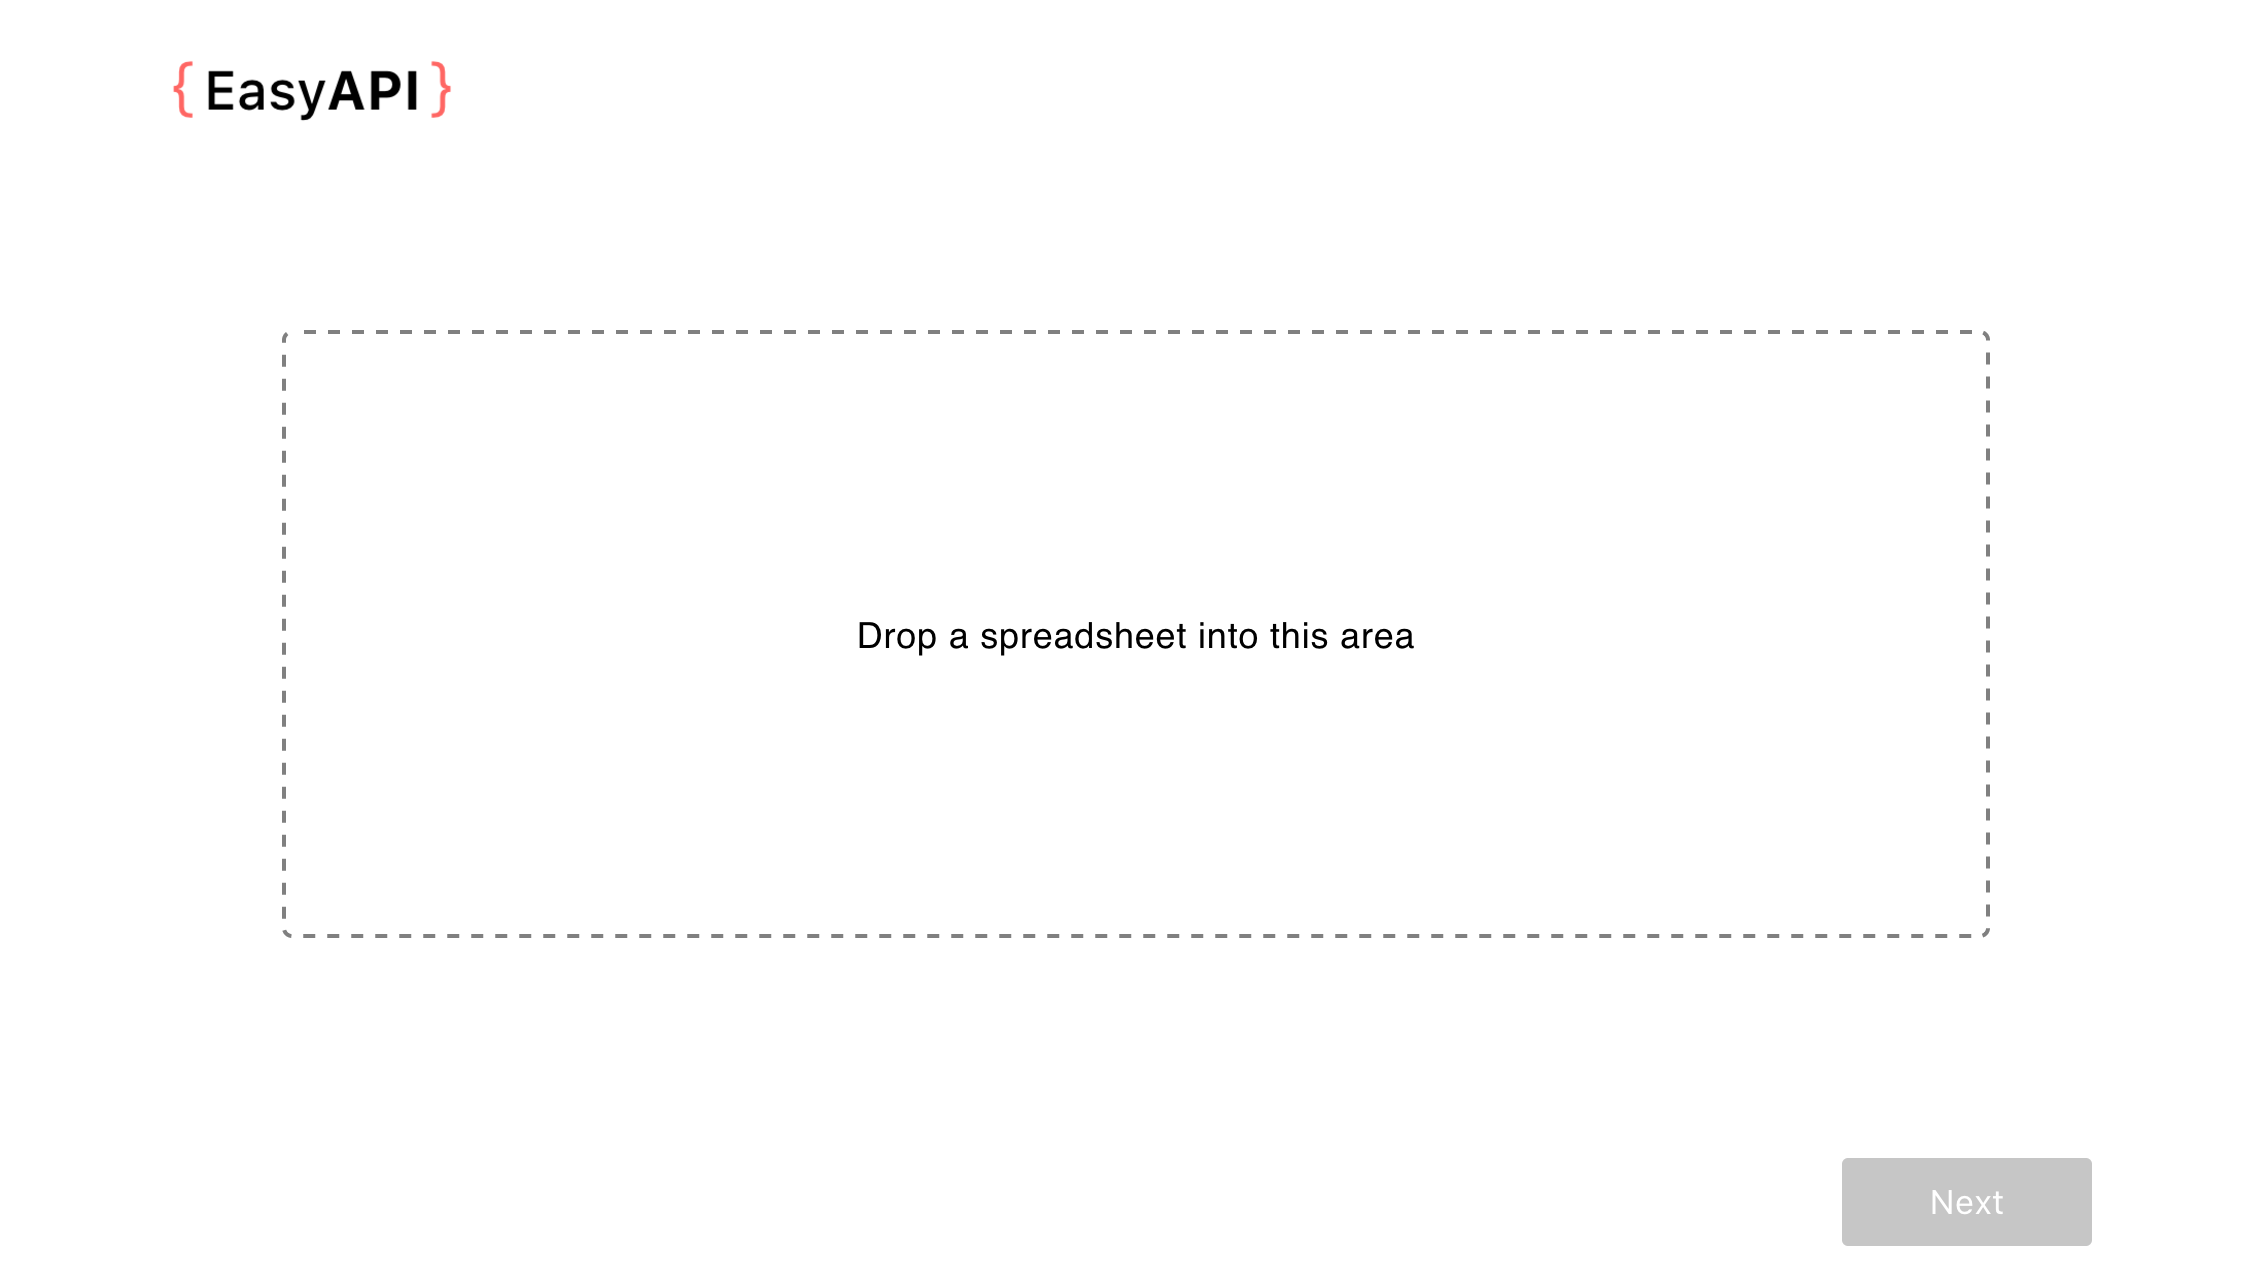
\includegraphics[scale=0.4]{screenshots/sheet.png}}
\caption{Spreadsheet upload screen}
\end{figure}




\subsection{Dashboard screen}
Once you have finished creating your API, you will be transferred to the dashboard screen. Through this screen you will be able to modify various aspects of your API.

On the right of the screen there is a sidebar through which you can navigate to other dashboard screens. In the centre-right of the screen you will see the content of the page you have currently selected.


\begin{figure}
\label{structure img}
\centerline{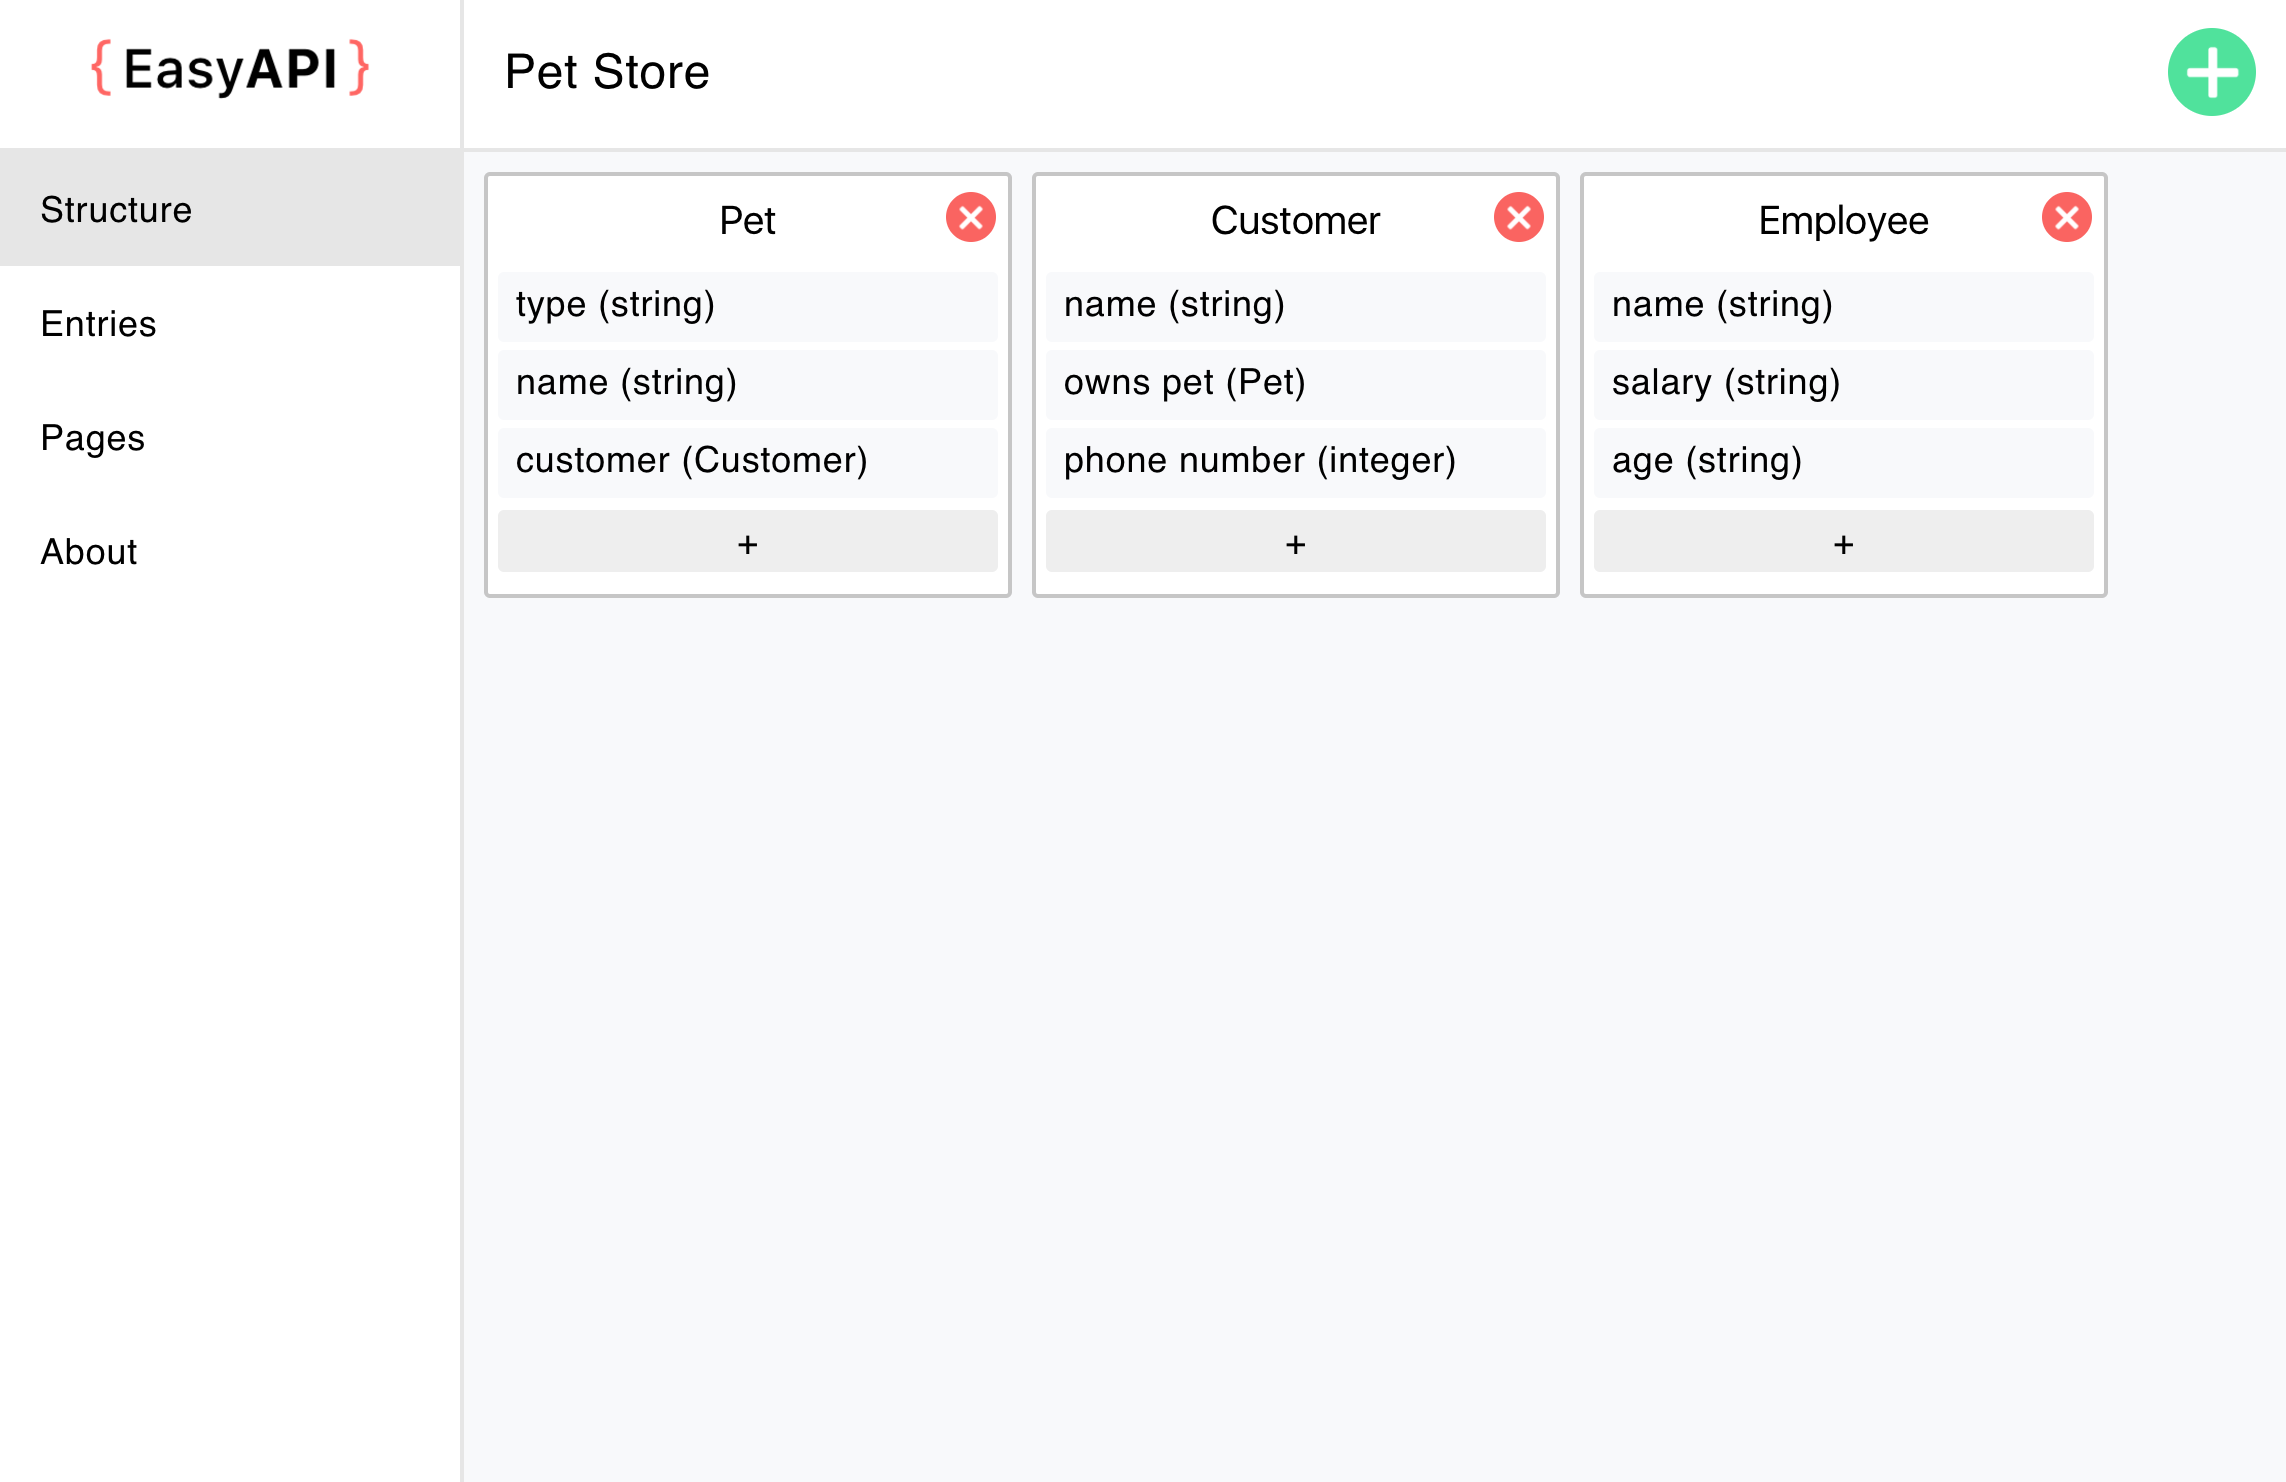
\includegraphics[scale=0.4]{screenshots/structure.png}}
\caption{Dashboard structure screen}
\end{figure}




\subsection{Modifying the database structure}

We will first look at how we can change our database structure. Here you can modify the underlying model definition, which defines how the database is structured.

Initially you will see boxes representing the various existing entities in your database. Each box will have a list of attributes for that entity.

If you decide to create a new entity to store in the database, click on the green plus button on the top of the screen.

To modify the name of an entity, select the title of an entity-box and type in the new entity name.

To modify an attribute of an entity, click on the specific attribute you want to edit. This will open a dialogue box which will present a number of fields for that attribute and let you modify it.

To delete an entity, click on the red button in a model box.

\begin{figure}
\label{attrimg}
\centerline{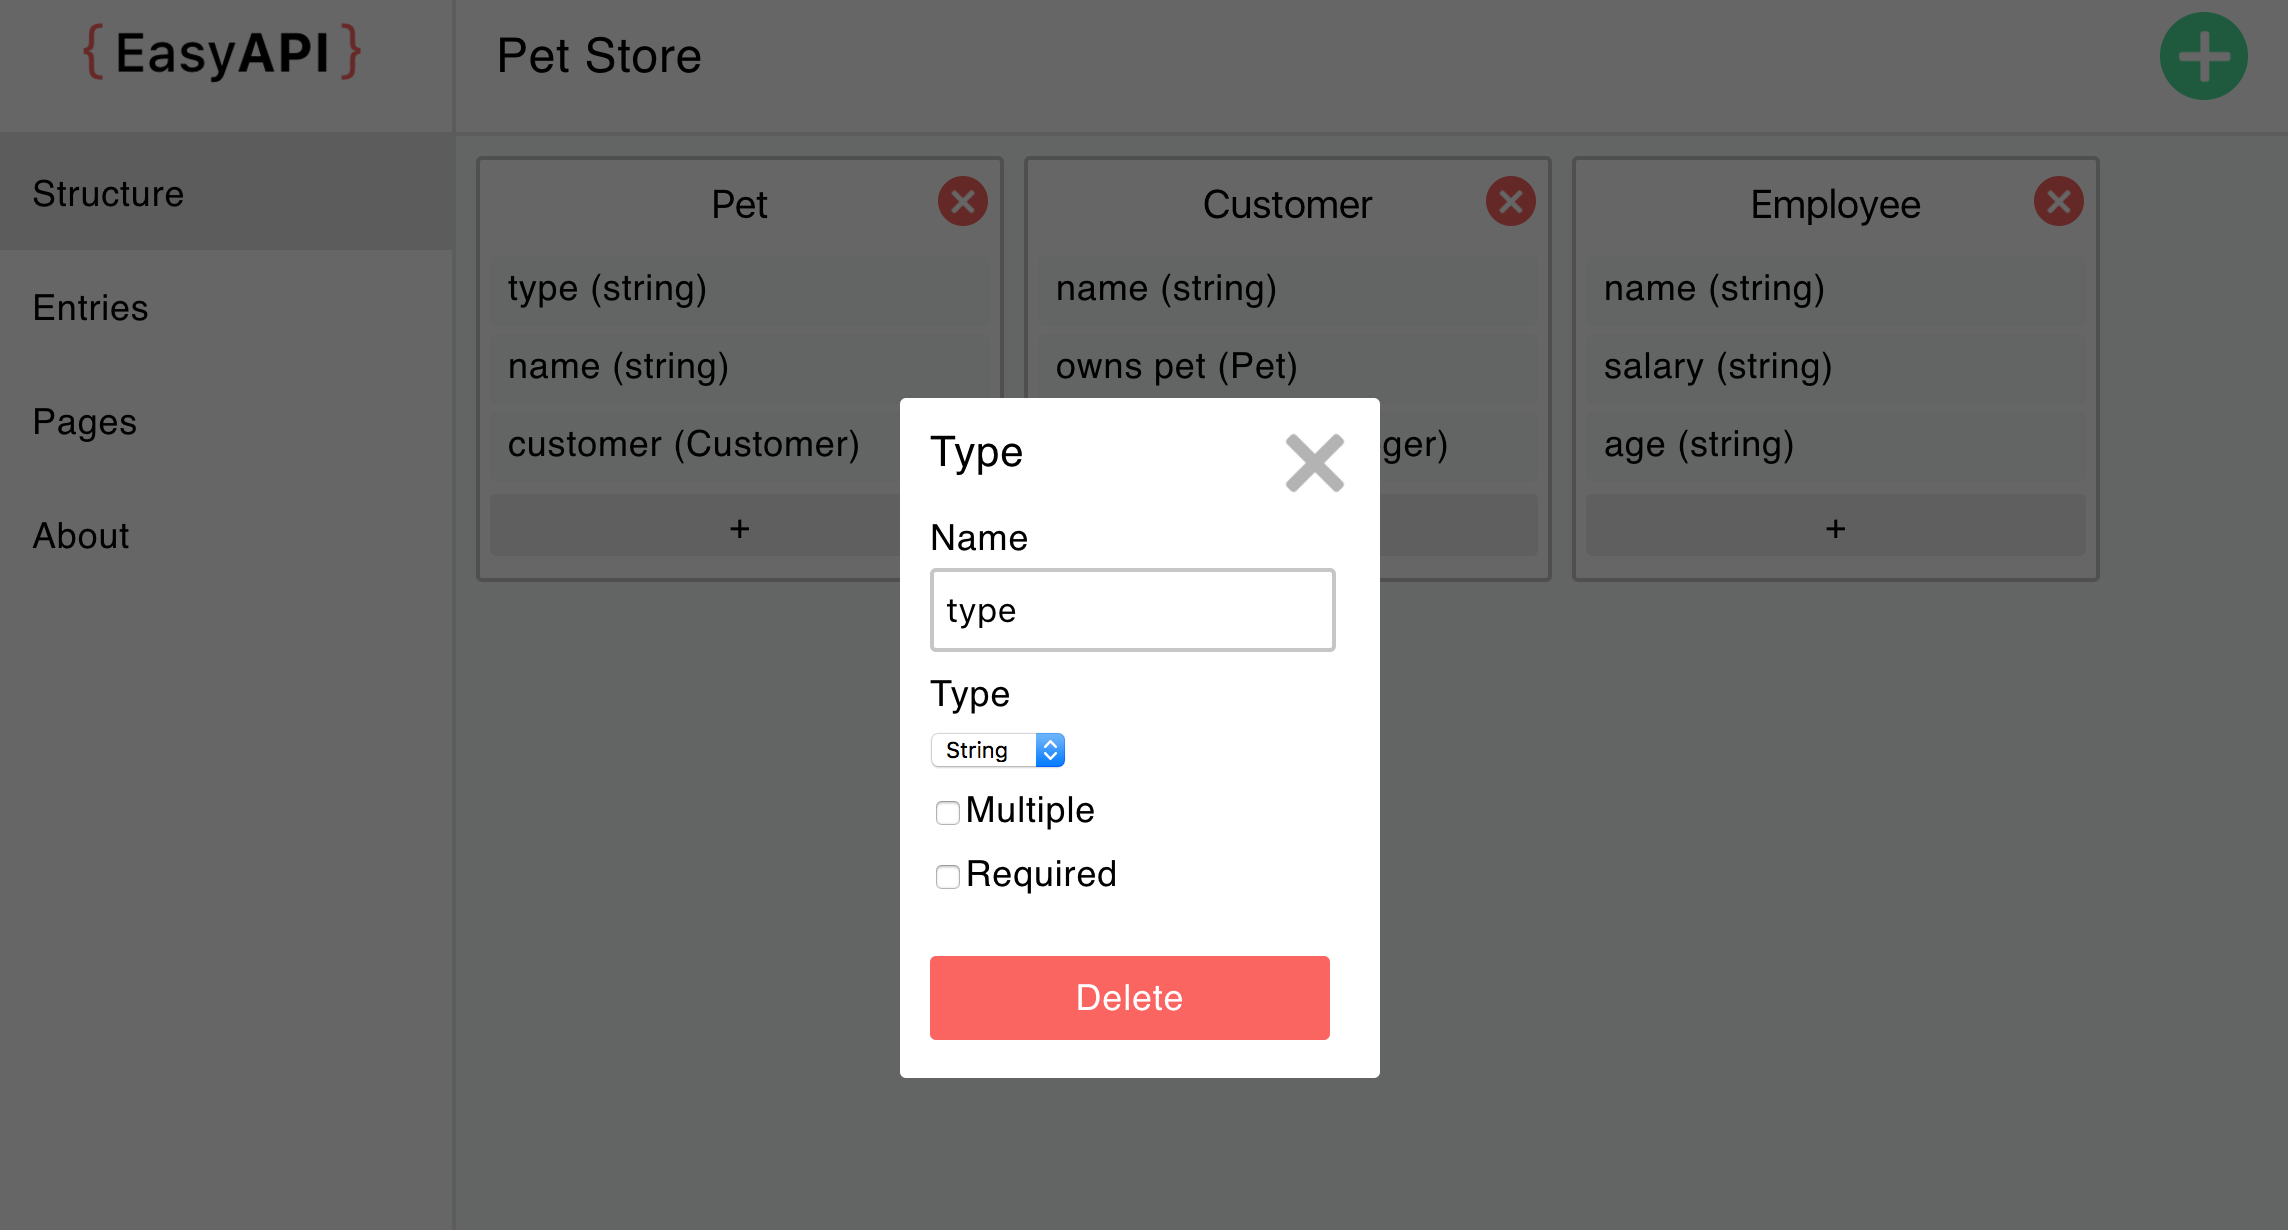
\includegraphics[scale=0.4]{screenshots/attr.png}}
\caption{Modify attribute dialog box}
\end{figure}



\subsection{Modifying the database entries}
The dashboard screen also allows you to manually modify the data in your database. Start by clicking on the "Entities" list item in the sidebar.

Your database is presented through a spreadsheet-like format. On the top of the screen you will see tabs for your corresponding entities. By clicking on each tab, the corresponding table will be shown.

To edit a value, simply click on it and type the new value. Be aware that it needs to conform to the defined type.

To delete an entry, click on red button which appears on the right to delete the row.

To create a new entry, click on the green button on the top of the screen and fill in the values in the row.


\begin{figure}
\label{entriesimg}
\centerline{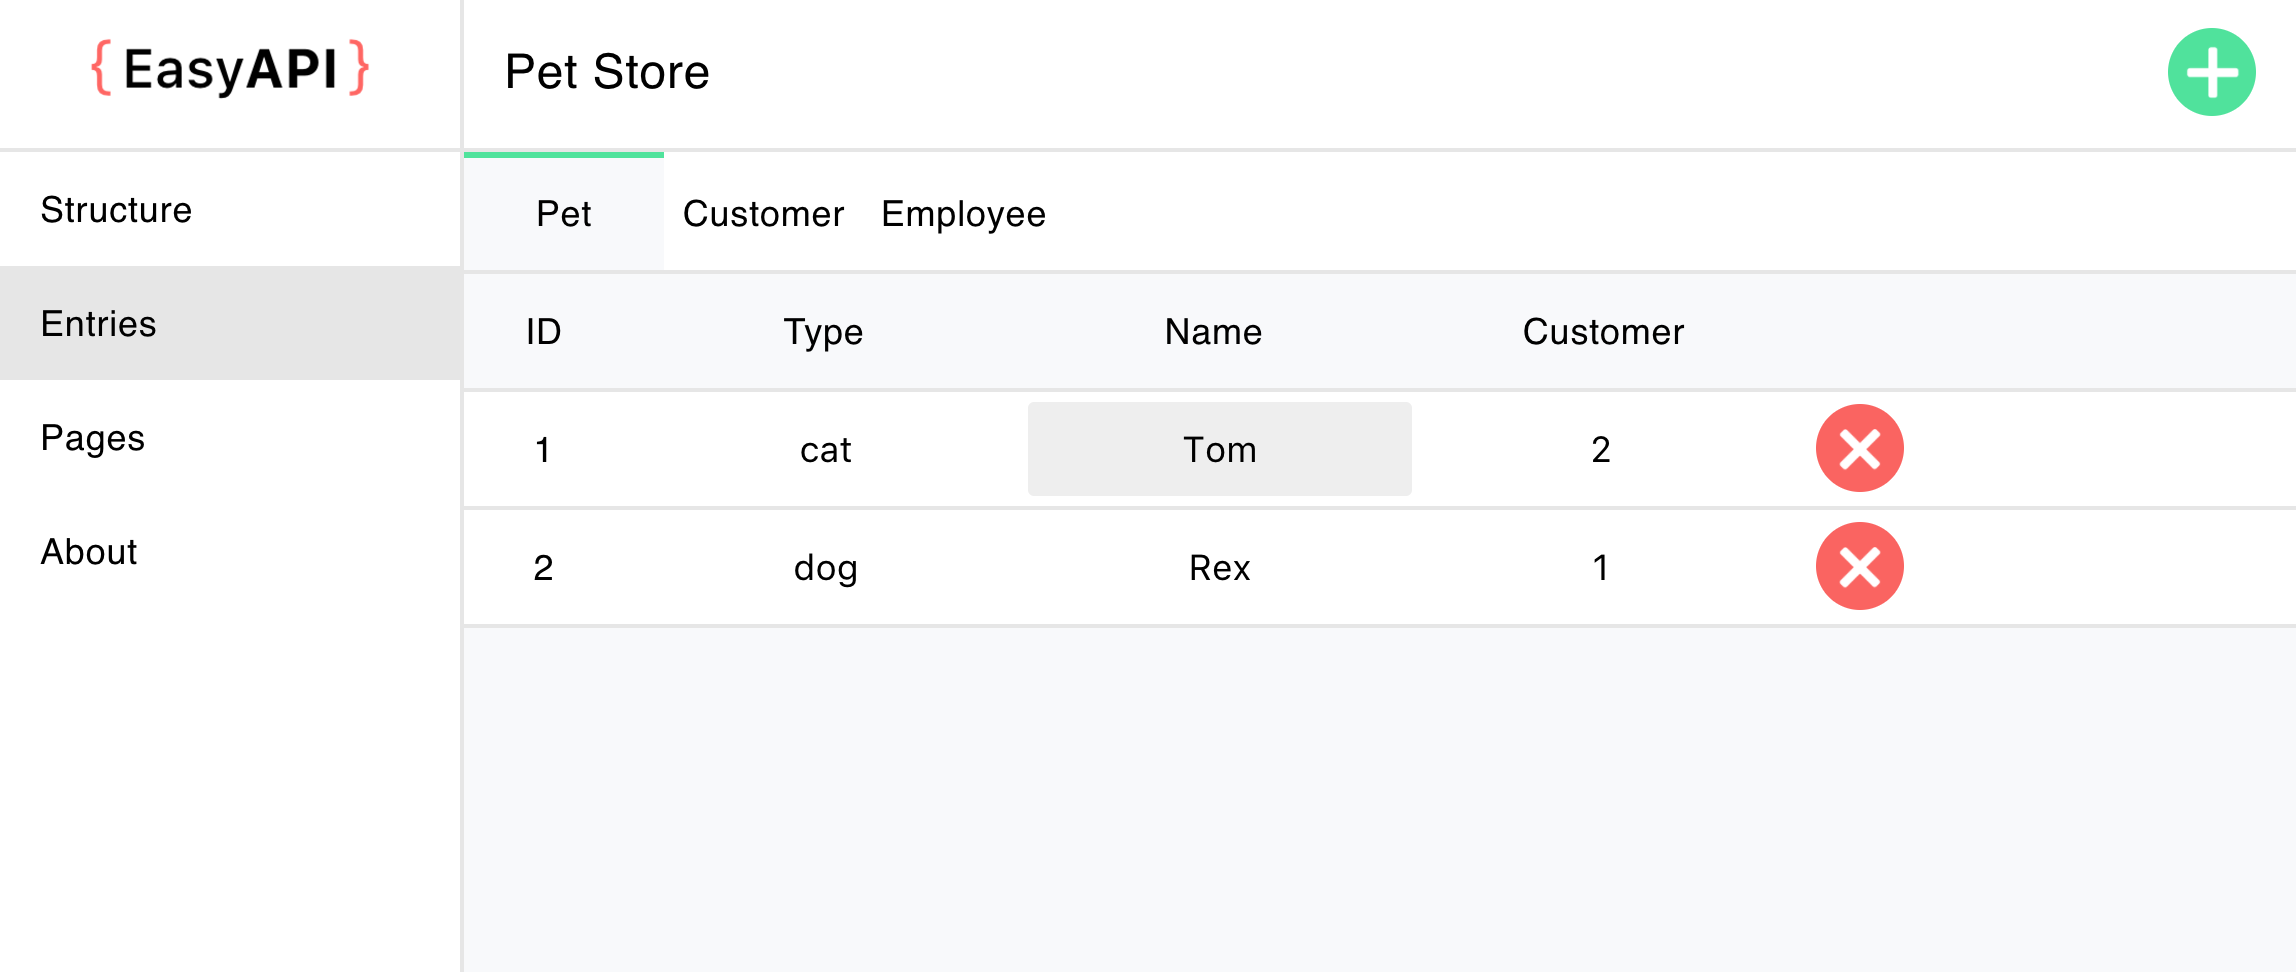
\includegraphics[scale=0.4]{screenshots/entries.png}}
\caption{Entries screen}
\end{figure}

\subsection{Modifying your public pages}
The "Pages" screen in the dashboard screen gives you control over which actions will be available to the public. Upon opening this page, you will see a list of your entities, each with a list of actions with check-boxes.

There are five optional actions for each entity:

\begin{itemize}
  \item \textbf{Find One}: This action is used to retrieve data of one resource on the server. It corresponds to the HTTP method GET.
  \item \textbf{Find}: This action is similar to the one above, except it is used to retrieve a list of resources.
  \item \textbf{Create}: This action is used to add a new entry to the database. It corresponds the the ``POST'' HTTP method.
  \item \textbf{Update}: This action allows users to modify existing resources and it corresponds to the PATCH HTTP action. Note that it does not correspond to the PUT HTTP action, as the request only requires the attributes to be updated.
  \item \textbf{Delete}: This action is used to delete an entry from the database.
\end{itemize}

To make a page available to the public, simply tick the checkbox next to an action. The URL of the endpoint will appear below.

\begin{figure}
\label{pagesimg}
\centerline{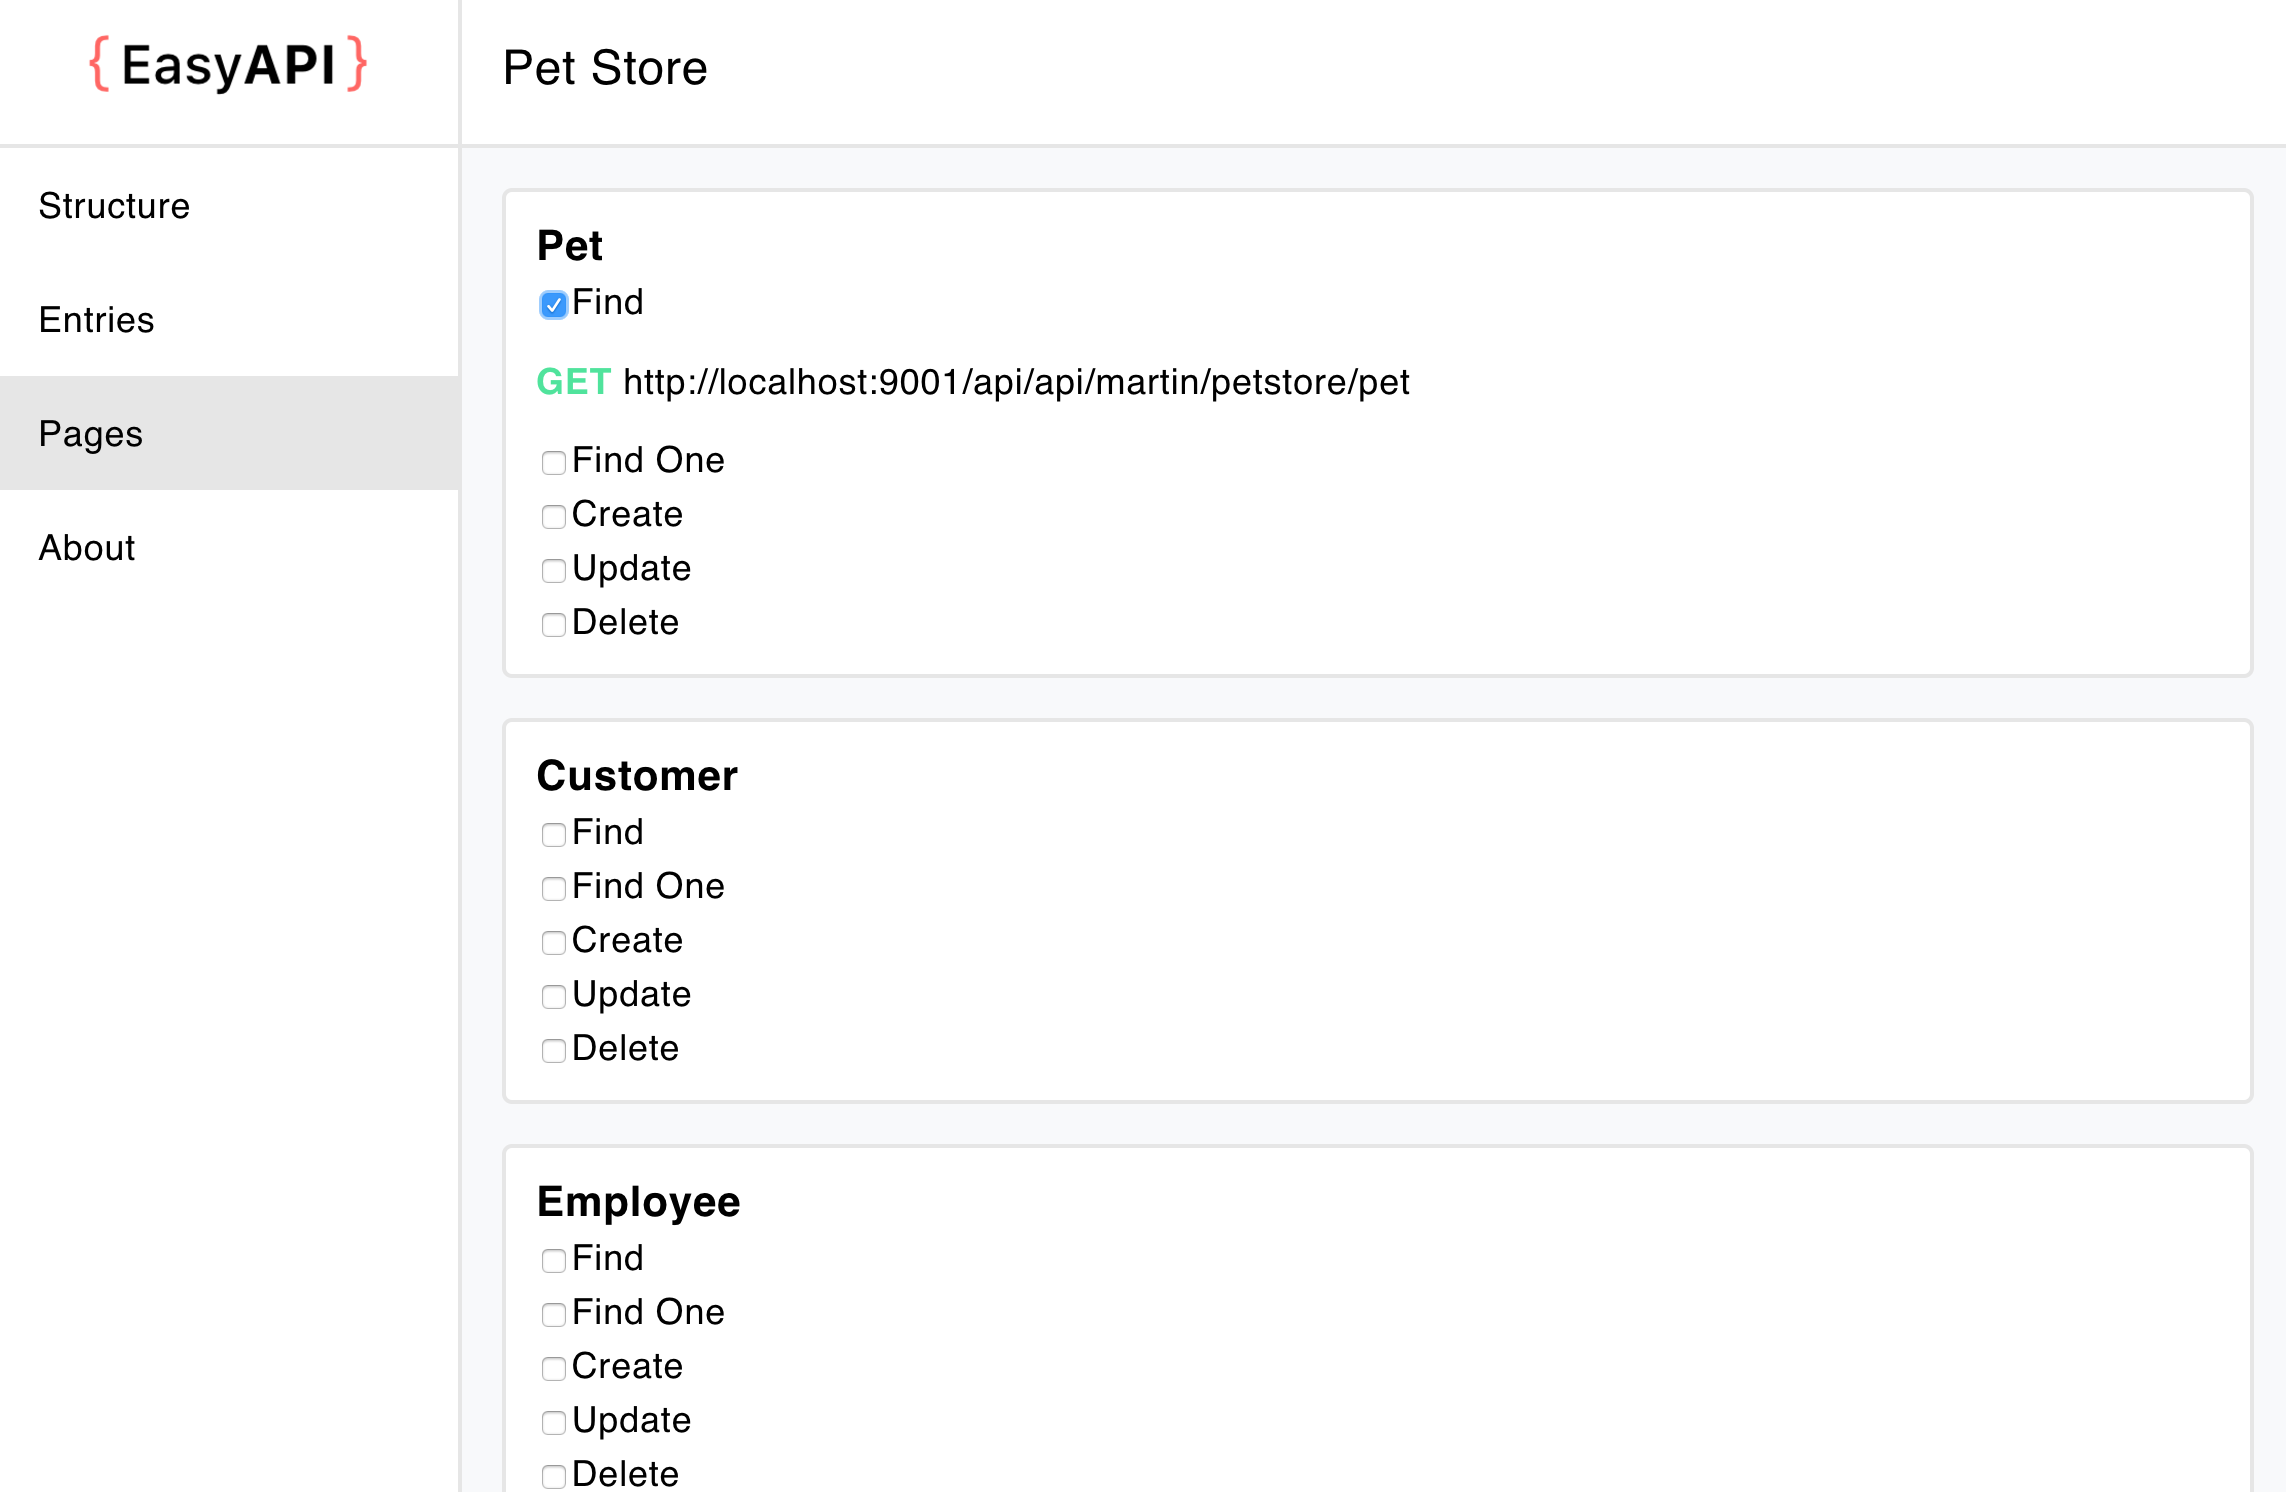
\includegraphics[scale=0.4]{screenshots/pages.png}}
\caption{Pages screen}
\end{figure}

\subsection{Modifying metadata and publishing}
Finally, you can also edit the metadata of the API and publish it.

You will find this screen by clicking on "About" in the sidebar.

To modify the name of the API, select the text field with the "Name" label and type your new name.

To modify the URL of the API, select the text field with the "URL" label and type in the new identifier for the API.

To publish your API, tick the checkbox next to the label "Public". You can unpublish it by un-ticking this checkbox.

\begin{figure}
\label{aboutimg}
\centerline{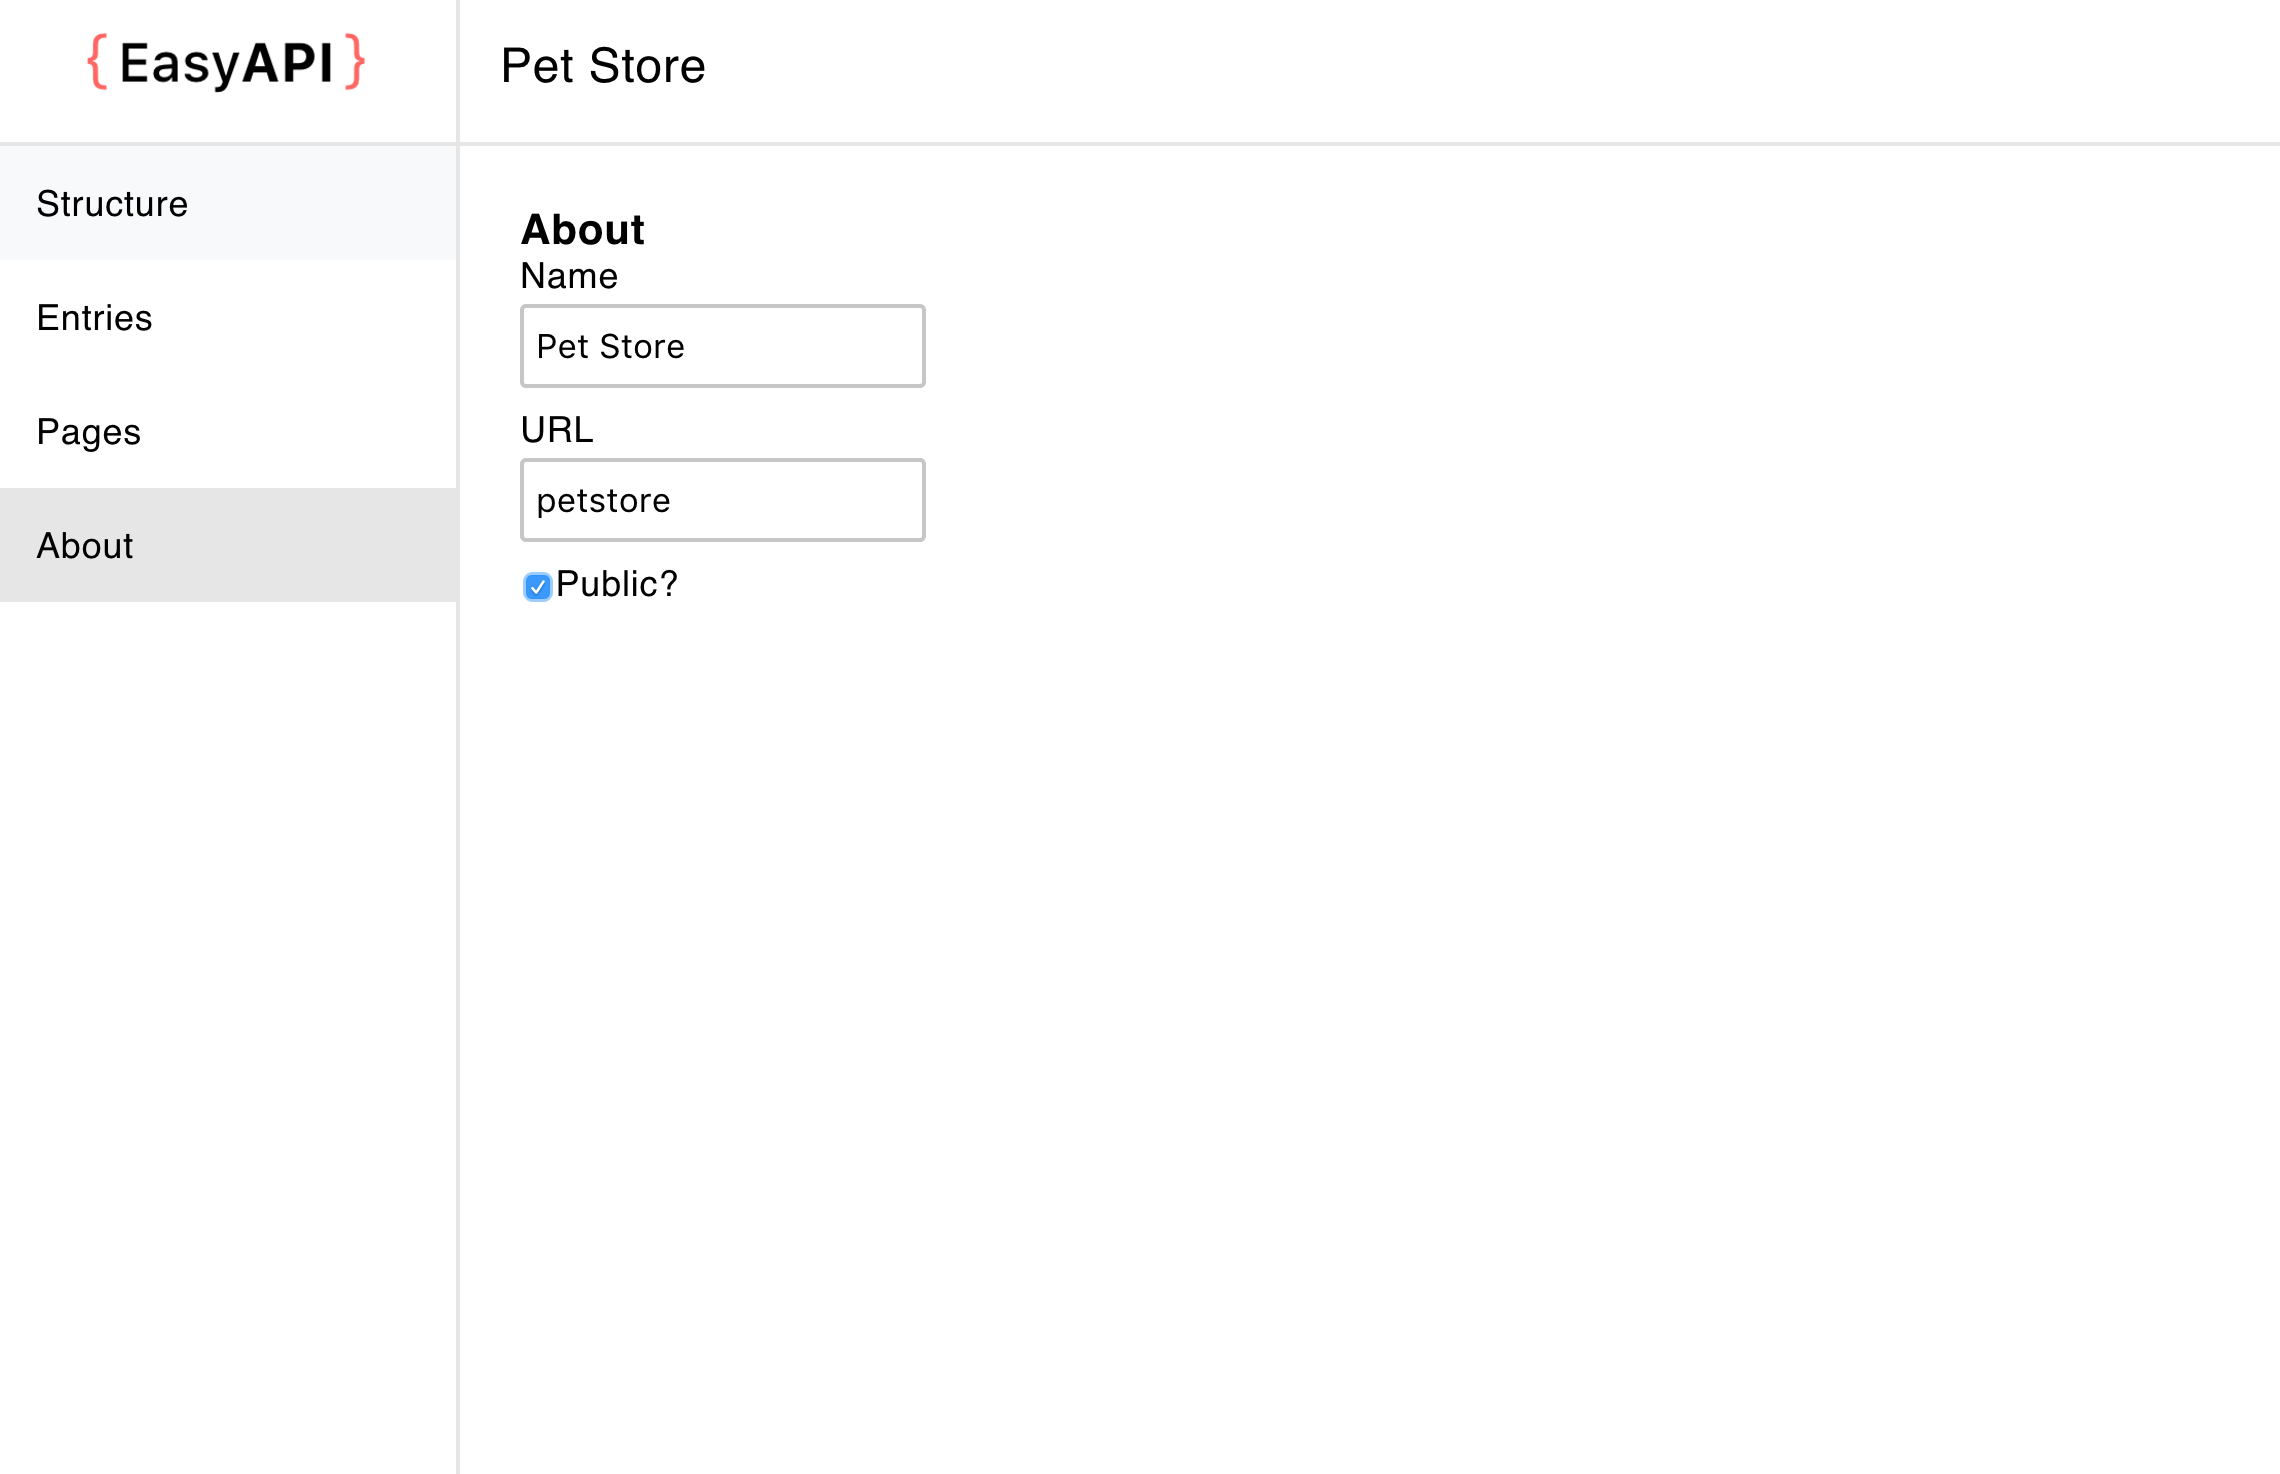
\includegraphics[scale=0.4]{screenshots/about.png}}
\caption{About screen}
\end{figure}

\subsection{Accessing your API}

After you publish your API, the first thing you might want to do is to test it out. You can do so by returning to the "Pages" screen, where you will see URLs under every enabled action. These are in the form of URL templates, where variables in curly brackets should be replaced by a value. For instance if a URL is the following:

http://localhost:9001/api/api/petstore/cats/{id}

You should replace ``{id}'' with an entry id. For certain actions where a request body is required, you will need to use a tool such as \href{https://www.getpostman.com/}{Postman} to make a request.

\begin{figure}
\label{rest}
\centerline{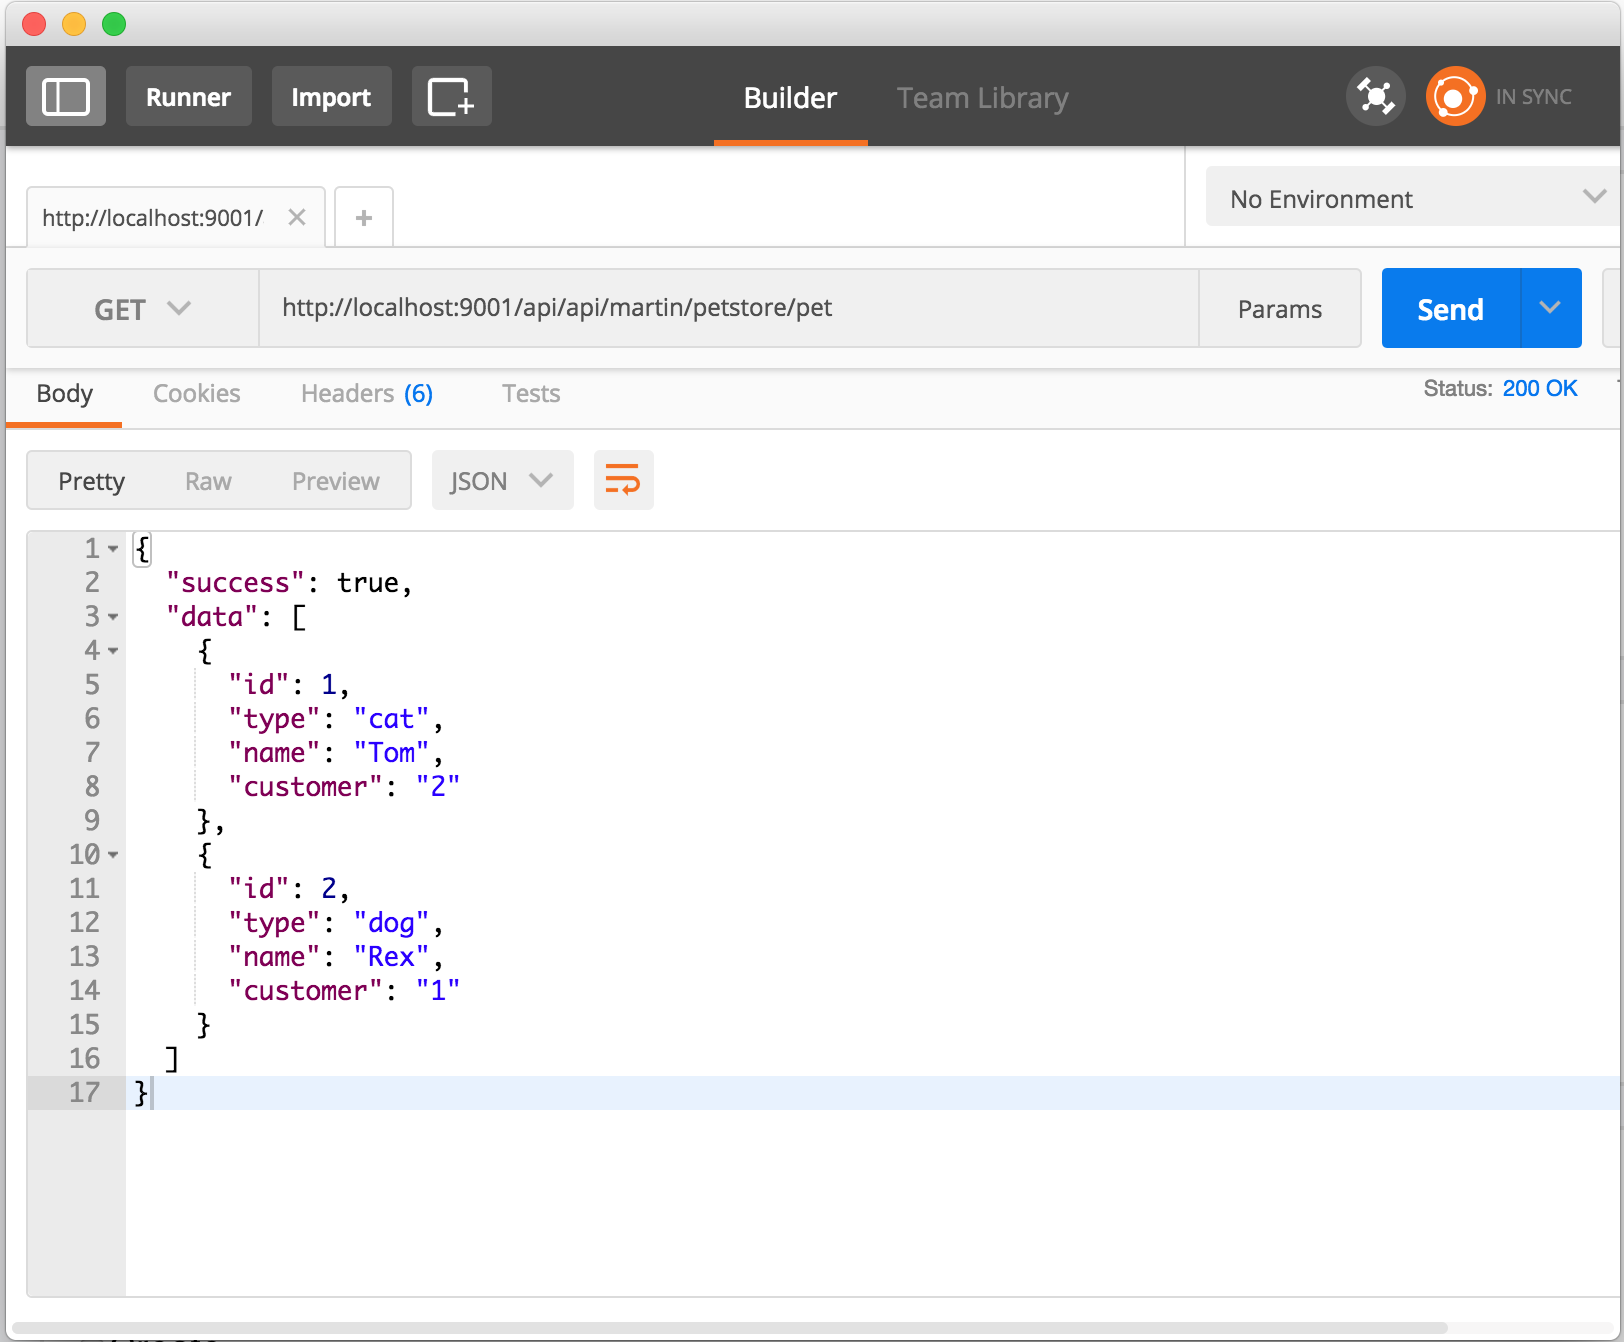
\includegraphics[scale=0.4]{screenshots/api.png}}
\caption{Accessing API through Postman}
\end{figure}
By making a request to the specified URL with the correct HTTP action and body, you should see the expected results. For the POST and PATCH actions, the body should be specified in JSON format.
